\documentclass{aims}
%DIF LATEXDIFF DIFFERENCE FILE
%DIF DEL DFSE_Lynch_original.tex   Sat Oct 24 11:29:48 2026
%DIF ADD DFSE_Lynch.tex            Sun Oct 25 17:11:18 2026


\usepackage{txfonts}
\def\typeofarticle{Research article}
\def\currentvolume{X}
\def\currentissue{x}
\def\currentyear{2026}
\def\currentmonth{Received: xxx; Accepted: xxx; Published: xxx}
\def\ppages{xxx--xxx}
\def\DOI{}
\def\Received{}
\def\Revised{}
\def\Accepted{}
\def\Published{}
%%%%%%%%%%%%%%%%
\usepackage[round,authoryear]{natbib}

\usepackage{lineno}
% Ensure display equations are line-numbered too (lineno skips amsmath math by
% default, which would leave gaps in the numbering around equations).
\newcommand*\patchAmsMathEnvironmentForLineno[1]{%
  \expandafter\let\csname old#1\expandafter\endcsname\csname #1\endcsname
  \expandafter\let\csname oldend#1\expandafter\endcsname\csname end#1\endcsname
  \renewenvironment{#1}%
    {\linenomath\csname old#1\endcsname}%
    {\csname oldend#1\endcsname\endlinenomath}}%
\newcommand*\patchBothAmsMathEnvironmentsForLineno[1]{%
  \patchAmsMathEnvironmentForLineno{#1}%
  \patchAmsMathEnvironmentForLineno{#1*}}%
\AtBeginDocument{%
  \patchBothAmsMathEnvironmentsForLineno{equation}%
  \patchBothAmsMathEnvironmentsForLineno{align}%
  \patchBothAmsMathEnvironmentsForLineno{gather}%
  \patchBothAmsMathEnvironmentsForLineno{multline}%
}
\usepackage{booktabs}
\numberwithin{equation}{section}
\makeatletter
\renewcommand{\@biblabel}[1]{}
\makeatother
%DIF PREAMBLE EXTENSION ADDED BY LATEXDIFF
%DIF UNDERLINE PREAMBLE %DIF PREAMBLE
\RequirePackage[normalem]{ulem} %DIF PREAMBLE
\RequirePackage{color}\definecolor{RED}{rgb}{1,0,0}\definecolor{BLUE}{rgb}{0,0,1} %DIF PREAMBLE
\providecommand{\DIFadd}[1]{{\protect\color{blue}\uwave{#1}}} %DIF PREAMBLE
\providecommand{\DIFdel}[1]{{\protect\color{red}\sout{#1}}}                      %DIF PREAMBLE
%DIF SAFE PREAMBLE %DIF PREAMBLE
\providecommand{\DIFaddbegin}{} %DIF PREAMBLE
\providecommand{\DIFaddend}{} %DIF PREAMBLE
\providecommand{\DIFdelbegin}{} %DIF PREAMBLE
\providecommand{\DIFdelend}{} %DIF PREAMBLE
\providecommand{\DIFmodbegin}{} %DIF PREAMBLE
\providecommand{\DIFmodend}{} %DIF PREAMBLE
%DIF FLOATSAFE PREAMBLE %DIF PREAMBLE
\providecommand{\DIFaddFL}[1]{\DIFadd{#1}} %DIF PREAMBLE
\providecommand{\DIFdelFL}[1]{\DIFdel{#1}} %DIF PREAMBLE
\providecommand{\DIFaddbeginFL}{} %DIF PREAMBLE
\providecommand{\DIFaddendFL}{} %DIF PREAMBLE
\providecommand{\DIFdelbeginFL}{} %DIF PREAMBLE
\providecommand{\DIFdelendFL}{} %DIF PREAMBLE
%DIF COLORLISTINGS PREAMBLE %DIF PREAMBLE
\RequirePackage{listings} %DIF PREAMBLE
\RequirePackage{color} %DIF PREAMBLE
\lstdefinelanguage{DIFcode}{ %DIF PREAMBLE
%DIF DIFCODE_UNDERLINE %DIF PREAMBLE
  moredelim=[il][\color{red}\sout]{\%DIF\ <\ }, %DIF PREAMBLE
  moredelim=[il][\color{blue}\uwave]{\%DIF\ >\ } %DIF PREAMBLE
} %DIF PREAMBLE
\lstdefinestyle{DIFverbatimstyle}{ %DIF PREAMBLE
	language=DIFcode, %DIF PREAMBLE
	basicstyle=\ttfamily, %DIF PREAMBLE
	columns=fullflexible, %DIF PREAMBLE
	keepspaces=true %DIF PREAMBLE
} %DIF PREAMBLE
\lstnewenvironment{DIFverbatim}{\lstset{style=DIFverbatimstyle}}{} %DIF PREAMBLE
\lstnewenvironment{DIFverbatim*}{\lstset{style=DIFverbatimstyle,showspaces=true}}{} %DIF PREAMBLE
%DIF END PREAMBLE EXTENSION ADDED BY LATEXDIFF

\begin{document}


\title{\DIFdelbegin \DIFdel{Diagnosing and mitigating the neutral-class deficit in financial sentiment analysis}\DIFdelend \DIFaddbegin \DIFadd{In-domain adaptation of FinBERT to retail-investor social-media text}\DIFaddend : \DIFdelbegin \DIFdel{An }\DIFdelend \DIFaddbegin \DIFadd{A controlled test of }\DIFaddend explainability-guided \DIFdelbegin \DIFdel{approach on multi-source investor text}\DIFdelend \DIFaddbegin \DIFadd{data selection}\DIFaddend }

\author{%
  Dominic Hubble\affil{1}
  and
  Stephen Lynch\affil{1,}\corrauth
}

\shortauthors{D. Hubble and S. Lynch}

\address{%
  \addr{\affilnum{1}}{Department of Computer Science, Loughborough University, Loughborough, LE11 3TU, United Kingdom}}

\corraddr{Email: s.lynch@lboro.ac.uk; Tel: +44 (0)1509 225854. ORCID: \url{https://orcid.org/0000-0002-4183-5122}.}

\begin{abstract}
Domain-adaptive transformer models such as FinBERT \DIFdelbegin \DIFdel{dominate }\DIFdelend \DIFaddbegin \DIFadd{are widely used for }\DIFaddend financial
sentiment classification, \DIFdelbegin \DIFdel{yet they share a stubborn blind spot: they misread neutral, factual
statements as positive or negative, and this neutral-class weakness is almost always
reported as a bare error rate and never explained. We turn that weakness into
something diagnosable and fixable. Using a purpose-built 200-sample benchmark that
mirrors the noisy, multi-source reality of deployed financial text (retail
}\DIFdelend \DIFaddbegin \DIFadd{but they are typically trained and evaluated on curated,
professionally written text. We examine how FinBERT performs on the noisier text
that a deployed system ingests, retail-investor }\DIFaddend discussion on Reddit, \DIFdelbegin \DIFdel{microblog reactions }\DIFdelend \DIFaddbegin \DIFadd{posts }\DIFaddend on
X/Twitter \DIFdelbegin \DIFdel{, and professional news), we
first show that FinBERT beats a finance-lexicon baseline by 13.5 points of accuracy
and 12.4 points of macro F1, a gap that survives a paired McNemar test
($p = 0.002$) and non-overlapping stratified-bootstrap confidence intervals. Benchmark labels are validated by a large language model (LLM) cross-annotation pass
and an independent human annotator(Cohen's $\kappa = 0.99$ and $0.90$). We then use
}\DIFdelend \DIFaddbegin \DIFadd{and news, and whether a small amount of in-domain fine-tuning helps. On a
338-item benchmark sampled from the system's own multi-source database, with
model-assisted labels audited by a human annotator, stock FinBERT reaches a
macro-F1 of 0.498 and over-predicts the neutral class. We fine-tuned FinBERT on
three 900-item training arms, each over five seeds. Two arms share a 600-item
positive/negative base and differ only in their neutral examples: one uses neutral
text containing sentiment-loaded vocabulary, a selection motivated by }\DIFaddend local
interpretable model-agnostic explanations (LIME)\DIFdelbegin \DIFdel{not as a dashboard feature
but as a diagnostic instrument, pinpointing a single systematic failure mode:
contextually neutral risk words such as ``cautious'' and ``inflation'' are pushed to the negative class. Guided by this diagnosis, a deliberately small (300-sample) fine-tuning intervention on neutral-but-lexically-loaded text lifts neutral recall by
18.4 points (to 71.7\% ) }\DIFdelend \DIFaddbegin \DIFadd{, and the other uses randomly
chosen neutral text as a control. Mean macro-F1 rose to 0.591 for the LIME-guided
arm and 0.607 for the random-neutral arm, gains of 9.3 }\DIFaddend and \DIFdelbegin \DIFdel{overall accuracy to 86.5\%, with no loss on the polarised classes. The
contribution is methodological: an explainability-guided loop
that closes the gap between diagnosing a model error and repairing it, validated on
realistic multi-source text with the paired significance testing that applied
sentiment studies too often omit}\DIFdelend \DIFaddbegin \DIFadd{11.0 points over stock
FinBERT that hold under an item-level paired bootstrap with Holm correction
(adjusted $p = 0.004$ and $p < 0.001$). A third, mixed arm (0.534) gave no reliable
gain. LIME-guided selection did not outperform the random control (difference
$-1.6$ points, 95\% CI $[-5.0, +1.7]$). Out of domain, every fine-tuned model scored
below stock FinBERT on Financial PhraseBank and on Twitter Financial News (for
example, macro-F1 0.630 against 0.668 on the latter for the random-neutral arm). The
results support modest in-domain adaptation, not improved general-purpose
classification, and show the value of testing explanation-derived hypotheses
against a matched control}\DIFaddend .
\end{abstract}

\DIFdelbegin %DIFDELCMD < \keywords{financial sentiment analysis; FinBERT; explainable AI; LIME; neutral-class recall; domain adaptation; targeted fine-tuning; investor sentiment; multi-source text; model error analysis
%DIFDELCMD < \newline
%DIFDELCMD < \textbf{JEL Codes:} C45, C52, C53, G14, G17, G41}
%DIFDELCMD < %%%
\DIFdelend \DIFaddbegin \keywords{financial sentiment analysis; FinBERT; explainable AI; LIME; domain adaptation; fine-tuning; social media; investor sentiment; multi-source text; model error analysis
\newline
\textbf{JEL Codes:} C45, C52, C53, G14, G17, G41}
\DIFaddend 

\maketitle
\linenumbers

\section{Introduction}
% =====================================================================
Markets do not move on facts alone; they move on how investors read those facts.
Investor sentiment is a well-documented driver of asset prices, trading volume and
volatility, capable of producing temporary mispricings that persist until
information is absorbed \citep{tetlock2007,baker2006}. The migration of investor
discourse onto social media and online communities has made it possible to
quantify this sentiment at scale, and domain-adaptive transformer models, chiefly
FinBERT \citep{araci2019}, have become \DIFdelbegin \DIFdel{the }\DIFdelend \DIFaddbegin \DIFadd{a }\DIFaddend standard tool for doing so, capturing
implicit financial phrasing (``guidance raised'', ``missed expectations'', ``strong
headwinds'') that earlier lexicon and bag-of-words methods cannot.

\DIFdelbegin \DIFdel{A recurring and well-documented limitation of FinBERT is its weak performance on the }\DIFdelend \DIFaddbegin \DIFadd{FinBERT was, however, fine-tuned on curated financial news sentences, and its
behaviour on retail-investor social-media posts, which are shorter, more informal
and differently balanced across classes, is less well characterised. Its handling
of the }\DIFaddend \emph{neutral} \DIFdelbegin \DIFdel{class: the model is biased toward the polarised classes on which its pre-training corpus is richest, and routinely mislabels factual, sentiment-free statements as positive or negative. This limitation is almost
always reported as a number (a low neutral recall or a confusion-matrix row) and
left there. What is missing is a }\emph{\DIFdel{mechanistic}} %DIFAUXCMD
\DIFdel{account of }\emph{\DIFdel{why}} %DIFAUXCMD
\DIFdel{the model fails on neutral text , 
as well as evidence that this failure is }\emph{\DIFdel{addressable}} %DIFAUXCMD
\DIFdel{with a proportionate intervention}\DIFdelend \DIFaddbegin \DIFadd{class is a frequently reported weakness, but the direction
and size of neutral-class errors depend on the text distribution and the labelling
conventions used}\DIFaddend . Existing surveys of explainable AI (XAI) in finance \DIFdelbegin \DIFdel{note a parallel gap: }\DIFdelend \DIFaddbegin \DIFadd{also note
that }\DIFaddend interpretability methods are \DIFdelbegin \DIFdel{overwhelmingly used either }\DIFdelend \DIFaddbegin \DIFadd{mostly used }\DIFaddend for post-hoc presentation or \DIFdelbegin \DIFdel{for offline
auditing ,
rather than as instruments that feed back into }\DIFdelend \DIFaddbegin \DIFadd{offline
auditing rather than to inform }\DIFaddend model improvement \citep{yeo2025}\DIFaddbegin \DIFadd{, and such uses are
rarely tested against a control}\DIFaddend .

This paper \DIFdelbegin \DIFdel{closes that loop. Our central claim is that FinBERT's neutral-class
deficit is not diffuse noise but a }\emph{\DIFdel{specific, lexically-localised, and
repairable}} %DIFAUXCMD
\DIFdel{failure mode, and that a local interpretability method can be used to
diagnose it precisely enough to motivate a targeted, measurable fix. Concretely,
we }\DIFdelend \DIFaddbegin \DIFadd{asks two questions. First, does a small amount of in-domain fine-tuning
improve FinBERT on the multi-source text that a deployed system actually ingests?
Second, does choosing fine-tuning data on the basis of local explanations help more
than choosing it at random? We }\DIFaddend make the following contributions:
\begin{enumerate}
\item \textbf{A \DIFdelbegin \DIFdel{realistic }\DIFdelend multi-source \DIFaddbegin \DIFadd{evaluation }\DIFaddend benchmark\DIFdelbegin \DIFdel{and a rigorous baseline
comparison}\DIFdelend .} We construct a \DIFdelbegin \DIFdel{200-sample financial-sentiment benchmark
reflecting
the true mixture of retail, microblog }\DIFdelend \DIFaddbegin \DIFadd{338-item benchmark
sampled from a deployed system's database of Reddit, X/Twitter }\DIFaddend and news text\DIFdelbegin \DIFdel{that a deployed system
ingests, }\DIFdelend \DIFaddbegin \DIFadd{, with
model-assisted labels under a written rubric and a human audit. On it, stock FinBERT
reaches a macro-F1 of 0.498 and over-predicts the neutral class (228 neutral
predictions against 135 gold neutral items).
}\item \textbf{\DIFadd{A controlled in-domain fine-tuning comparison.}} \DIFadd{We fine-tune FinBERT on
three 900-item arms over five seeds each and compare them with stock FinBERT using
paired tests with multiple-comparison correction. Mean macro-F1 rises to 0.591 }\DIFaddend and
\DIFdelbegin \DIFdel{we validate its labels with both large language model (LLM)cross-annotation and an
independent human annotator.
We compare FinBERT against a finance-lexicon keyword
baseline using
a }\emph{\DIFdel{paired}} %DIFAUXCMD
\DIFdel{significance test (McNemar) and stratified-bootstrap
confidence intervals, a level of statistical rigour that comparable applied studies
frequently omit}\DIFdelend \DIFaddbegin \DIFadd{0.607 for the two arms that share a positive/negative base (bootstrap gains of 9.3
and 11.0 points, Holm-adjusted $p = 0.004$ and $p < 0.001$), while a mixed arm
(0.534) gives no reliable gain}\DIFaddend .
\item \textbf{\DIFdelbegin \DIFdel{An explainability-guided diagnosis }\DIFdelend \DIFaddbegin \DIFadd{A test }\DIFaddend of \DIFdelbegin \DIFdel{the neutral-class deficit.}%DIFDELCMD < \MBLOCKRIGHTBRACE
%DIFDELCMD < %%%
\DIFdel{Using local interpretable model-agnostic explanations (LIME ) as a diagnostic
instrument rather than }\DIFdelend \DIFaddbegin \DIFadd{LIME-guided data selection against }\DIFaddend a \DIFdelbegin \DIFdel{user-facing feature, we show
that FinBERT 's neutral failures are driven by a
consistent mechanism: contextually
neutral risk vocabulary is systematically attributed to the negative class.
}\DIFdelend \DIFaddbegin \DIFadd{random control.}}
\DIFadd{LIME examples suggested that neutral text containing sentiment-loaded vocabulary
would be especially useful for fine-tuning. Selecting neutrals this way did not
outperform randomly selected neutrals (difference $-1.6$ points, 95\% CI
$[-5.0, +1.7]$), so we treat LIME here as hypothesis-generating rather than as the
source of the improvement.
}\DIFaddend \item \DIFdelbegin \textbf{\DIFdel{A targeted, evidence-led mitigation.}} %DIFAUXCMD
\DIFdel{Guided by the diagnosis, we
fine-tune on a small, disjoint corpus of neutral-but-lexically-loaded financial text and recover neutral recall by 18.4 percentage points while preserving
polarised-class performance, demonstrating that the diagnosed failure is
proportionately addressable}\DIFdelend \DIFaddbegin \textbf{\DIFadd{An out-of-domain check.}} \DIFadd{All fine-tuned models score below stock
FinBERT on Financial PhraseBank and Twitter Financial News. We report this as a
limitation: the gains are specific to the target distribution and are not a claim
of better general financial sentiment classification}\DIFaddend .
\end{enumerate}

These results were obtained within, and are reported alongside, a fully deployed analytics system. The system's additional components (a finance-emotion enrichment layer, a lightweight aspect extractor, and a sentiment-price correlation engine) are described for contextual completeness, and their evaluations, including negative and null findings, are reported transparently rather than presented as headline claims. The remainder of the paper is organised as follows. Section~\ref{sec:related}
reviews related work; Section~\ref{sec:data} describes the data;
Section~\ref{sec:method} sets out the methodology; Section~\ref{sec:results}
presents results; Section~\ref{sec:discussion} discusses implications and threats
to validity; and Section~\ref{sec:conclusion} concludes.

% =====================================================================
\section{Literature review}\label{sec:related}
% =====================================================================
\subsection{Sentiment, text and markets}
Behavioural finance establishes that sentiment and psychological factors produce
temporary, economically meaningful mispricings \citep{baker2006}. \citet{tetlock2007}
showed that negative language in financial news predicts short-term downward
pressure on returns with subsequent reversion; \citet{antweiler2004} had already
established that user-generated message-board text carries statistically
significant information about volatility, and \citet{schumaker2009} reported
comparable short-horizon predictive content in breaking financial news.
\citet{bollen2011} extended this to social
media at scale, deriving daily mood indices from Twitter that predicted Dow Jones
movements, while \citet{da2015} reached a similar conclusion from aggregate search
volumes, and \citet{garcia2013} showed news-sentiment effects are strongest during
recessions. More recent work documents the distinct behaviour of retail
communities: \citet{long2023} show that Reddit sentiment during the GameStop
episode diverged sharply from institutional news, and cryptocurrency markets
exhibit comparable retail-driven sensitivity to Twitter sentiment
\citep{kraaijeveld2020}. The collective implication is that single-source sentiment
signals are structurally incomplete, motivating multi-source measurement.

\subsection{From lexicons to domain-adaptive transformers}
Early financial sentiment systems relied on domain-specific lexicons;
\citet{loughran2011} demonstrated that general-purpose word lists misclassify
finance vocabulary and produced the finance-specific dictionary that remains the
standard lexicon baseline. Lexicon methods are transparent and fast but fail on
negation, implicit polarity and context-dependent phrasing. The transformer
architecture \citep{vaswani2017} and bidirectional pre-training \citep{devlin2019}
changed the field, and FinBERT \citep{araci2019} adapted this to finance by
pre-training on financial corpora, consistently outperforming general models and
lexicons on the Financial PhraseBank benchmark \citep{malo2014}. Parallel FinBERT
variants target financial communications and filings
\citep{yang2020,huang2023}, and very recent work continues to adapt these models, for
example, through pseudo-label test-time adaptation of FinBERT \citep{yang2026plta} and
sparse mixture-of-experts augmentation of LLM-based sentiment classifiers
\citep{li2026augment}.

Since 2023, LLMs have been applied to financial sentiment
with mixed but informative results. ChatGPT-based scores have been found to
outperform FinBERT on some benchmarks and to carry incremental return-predictive
information \citep{fatouros2023,lopezlira2023}, while other work shows LLM sentiment
is brittle under adversarial rephrasing \citep{leippold2023} and unreliable on
informal Reddit-register text \citep{deng2023}. Domain LLMs such as BloombergGPT
\citep{wu2023} demonstrate strong zero-shot performance but are not publicly
available, and generative models are increasingly trialled across financial decision
workflows beyond sentiment, for instance, in venture screening \citep{vismara2026}. The consensus is that LLMs have narrowed the per-sentence accuracy gap
with FinBERT on clean benchmarks but have not displaced it where latency, cost and
reproducibility are first-order constraints, which is the setting of this study.
Across this literature, the neutral class is repeatedly identified as the hardest
and least-studied category, but is rarely diagnosed or remediated directly.

\subsection{Explainable AI in finance: presentation versus diagnosis}
\citet{doshivelez2017} frame interpretability as explaining model behaviour in
human-understandable terms wherever objectives cannot be fully specified in
advance, which is almost always the case in finance. LIME \citep{ribeiro2016}
explains individual predictions by fitting a sparse linear surrogate over
perturbations of the input, identifying the tokens most responsible for a
prediction; Shapley additive explanations (SHAP) \citep{lundberg2017} provides
game-theoretic guarantees at higher computational cost. Surveys find that XAI in finance is dominated by post-hoc LIME and SHAP but that deployment within interactive tools, and use as a feedback
mechanism, remain rare \citep{yeo2025}. \citet{sravankumar2025} integrate XAI with
deep learning for sentiment-driven stock prediction. Two cautionary
results bound the claims that interpretability can support: perturbation-based
explanations can be adversarially fooled \citep{slack2020}, and intrinsically
interpretable models may be preferable in high-stakes settings \citep{rudin2019}.
We therefore use LIME strictly as a \emph{diagnostic aid}, a hypothesis-generating
instrument whose output is corroborated against the confusion matrix and an
intervention, rather than as a guarantee of correctness. The gap this paper
addresses is thus narrow and specific: the use of local interpretability to
\emph{diagnose a known model failure mode precisely enough to drive a targeted,
validated mitigation}, evaluated on realistic multi-source financial text.

% =====================================================================
\section{Data}\label{sec:data}
% =====================================================================
\subsection{Multi-source corpus}
The deployed system ingests text from three complementary channels via documented
official interfaces: Reddit (long-form discussion from finance subreddits, via
PRAW), X/Twitter (high-frequency reactions, via the official X API v2), and
financial news (professionally sourced articles, via NewsAPI). All collection is
restricted to publicly available text; author-identifying fields (handles, display
names, geolocation) are stripped at ingestion, so that each stored record contains
only sanitised text, a timestamp, a source identifier, and any resolved ticker
mentions. Duplicate and near-duplicate detection (content-hashing and TF-IDF
cosine similarity) and minimum-length thresholds are applied. At the time of
analysis, the corpus comprised more than 150{,}000 labelled records. We note a
material data-layer limitation up front: tightened X API v2 quotas during
2023 to 2024 bounded the Twitter subcorpus well below the Reddit and news
subcorpora, so the Twitter signal is treated as secondary and corroborated
throughout (see Section~\ref{sec:discussion}). The project received a favourable
ethical opinion from the Loughborough University Ethics Review Sub-Committee through
the University's ethical review system; full approval and consent details are given
in the Ethics statement.

\subsection{Evaluation benchmark and label validation}\label{sec:benchmark}
Existing benchmarks such as Financial PhraseBank \citep{malo2014} consist of
professionally written news sentences and do not reflect the informal, noisy
language the deployed system processes. We therefore constructed a \DIFdelbegin \DIFdel{purpose-built
200-sample benchmark
spanning the three ingestion channels,balanced across
classes: 70 positive (earnings beats,
guidance raises, upgrades), 70 negative (misses, downgrades, sell-offs), and 60 neutral (factual announcements, regulatory
disclosures, on-par results) . Primary ground-truth labels }\DIFdelend \DIFaddbegin \DIFadd{benchmark
(benchmark v2) directly from the system's database of ticker-tagged records
(159}{\DIFadd{,}}\DIFadd{081 records at the time of sampling). Records were cleaned (URLs removed,
whitespace normalised), restricted to sentence-scale texts of 60 to 500 characters
with a heuristic English filter, and de-duplicated on normalised text. An initial
sample of 300 items was drawn uniformly at random within each channel (100 Reddit,
100 news, 100 Twitter; fixed seed), without reference to any model output.
Items labelled out of scope in this draw were replaced by further random draws
from the same channel (16 drawn; 12 retained), and, because the random draw contained few negative items, a top-up of
negative-lexicon-matching items was added (60 drawn; 56 retained); this top-up is
the only non-random component of the benchmark and is recorded per item. After
removal of 21 items judged unjudgeable or out of scope, the frozen benchmark
contains 338 items (135 neutral, 122 positive, 81 negative; 108 Reddit, 115 news,
115 Twitter), of which 66 are flagged as low-information factual filler and retained
as neutral under the labelling rubric.
Post timestamps (the stored publication time, present for all 338 items) span
24 August 2017 to 13 August 2026: news items from 24 August 2017 to 15 July 2026,
Reddit items from 8 February 2021 to 13 August 2026, and Twitter items from 3 January
2022 to 6 April 2026. The class mix and ticker coverage per channel are reported in
Table~\ref{tab:source}.
}

\DIFadd{Labels }\DIFaddend were assigned by \DIFaddbegin \DIFadd{model-assisted labelling under a written rubric (rubric
v2), with human audit by }\DIFaddend one author (D.H.)\DIFdelbegin \DIFdel{, cross-referencing each example against the Financial PhraseBank
taxonomy for consistency. }%DIFDELCMD < 

%DIFDELCMD < %%%
\DIFdel{Because single-annotator labelling is a threat to validity, we validated the
labels
in two independent ways. First, a large language model, given only the 200 raw
texts with no access to the labels of }\DIFdelend \DIFaddbegin \DIFadd{. The rubric defines sentiment as the
investor view of the asset discussed and fixes boundary cases (price-move and chart
calls follow the stated direction; mixed price-target lists and factual filler are
neutral). On a held-out reserve audit of 31 classifiable items, not used for rubric
development, agreement between }\DIFaddend D.H. and \DIFdelbegin \DIFdel{instructed to apply the Financial
PhraseBank taxonomy, produced a second label set; agreement was 199/200 (}\DIFdelend \DIFaddbegin \DIFadd{the model-assisted labels was }\DIFaddend Cohen's
\DIFdelbegin \DIFdel{$\kappa = 0.9925$, SE $= 0.0075$) \mbox{%DIFAUXCMD
\citep{cohen1960} }\hskip0pt%DIFAUXCMD
. We interpret this conservatively
as an }\emph{\DIFdel{internal-consistency}} %DIFAUXCMD
\DIFdel{check rather than a human inter-rater coefficient,
because the model and that author share overlapping training distributions and the
figure will overstate a human study. Second, an independent human annotator,a
finance undergraduate with equity-research internship experience and no involvement
in the project,labelled a 100-sample stratified subset (34/33/33) under the same instructions. Agreement between }\DIFdelend \DIFaddbegin \DIFadd{$\kappa = 0.807$ \mbox{%DIFAUXCMD
\citep{cohen1960} }\hskip0pt%DIFAUXCMD
(87.1\% agreement). The original 200-item benchmark used in an earlier version of
this work was not sampled from the corpus and is no longer used for any reported
result.
}

\subsection{Fine-tuning corpus}\label{sec:ftcorpus}
\DIFadd{The 300-item fine-tuning corpus used in an earlier version of this study, and the
run behind its reported result, could not be recovered; all fine-tuning results
reported here are new. A candidate pool of 2}{\DIFadd{,}}\DIFadd{300 posts was drawn from the same
database with the same cleaning and length filters, excluding every benchmark item
by identifier and normalised text, in two fixed-seed draws (1}{\DIFadd{,}}\DIFadd{100 then 1}{\DIFadd{,}}\DIFadd{200
items; in each, roughly 36\% unrestricted random and 64\% matching at least one term
of the system's finance sentiment lexicon). All 2}{\DIFadd{,}}\DIFadd{300 candidates were labelled with
rubric v2 by the same model-assisted procedure: 979 positive, 593 neutral, 635
negative and 93 excluded as out of scope. To audit the label most relevant to this
study, }\DIFaddend D.H. \DIFdelbegin \DIFdel{and the human annotator was 93.0\% (Cohen's
$\kappa = 0.895$) ; three-way Fleiss' $\kappa$ \mbox{%DIFAUXCMD
\citep{fleiss1971} }\hskip0pt%DIFAUXCMD
across }\DIFdelend \DIFaddbegin \DIFadd{blind-relabelled a random sample of 30 candidates labelled neutral:
agreement was 23/30, and neutral precision was 23/29 (0.793) after removing one item
}\DIFaddend D.H. \DIFdelbegin \DIFdel{, the
human annotator and the model label set on the subset was 0.893. Both coefficients
fall in the ``almost perfect'' band \mbox{%DIFAUXCMD
\citep{landis1977}}\hskip0pt%DIFAUXCMD
, and the seven disagreements between the human annotator and D.
H. clustered on the neutral/positive boundary, consistent with the failure
mode analysed in Section~\ref{sec:results}. These checks support,
but do not fully
substitute for, }\DIFdelend \DIFaddbegin \DIFadd{judged out of scope (the remaining disagreements were 5 positive and 1
negative).
}

\DIFadd{Three training arms were built from this pool (Table~\ref{tab:arms}). All three share
an identical base of 300 positive and 300 negative items, sampled with a fixed seed
from labelled positives and negatives not used elsewhere in the arms. They differ
only in }\DIFaddend a \DIFdelbegin \DIFdel{multi-annotator panel }\DIFdelend \DIFaddbegin \DIFadd{300-item arm-specific component: (a)~}\emph{\DIFadd{lexicon-loaded neutrals}}\DIFadd{,
neutral items containing at least one term of the finance sentiment lexicon, the
vocabulary that the LIME analysis }\DIFaddend (Section~\DIFdelbegin \DIFdel{\ref{sec:discussion}) .
}%DIFDELCMD < 

%DIFDELCMD < \subsection{Fine-tuning corpus}\label{sec:ftcorpus}
%DIFDELCMD < %%%
\DIFdel{For the mitigation experiment (Section~\ref{sec:ftmethod}), we assembled a 300-sample corpus of financial text that is sentiment-neutral but lexically
sentiment-loaded, drawn from
regulatory filings (8-K, 10-Q excerpts) , central-bank
statements, and earnings-release language of
the kind that produces FinBERT's
residual neutral confusions. This corpus was held strictly }\DIFdelend \DIFaddbegin \DIFadd{\ref{sec:limemethod}) implicates in
neutral errors; (b)~}\emph{\DIFadd{random neutrals}}\DIFadd{, drawn at random from all labelled
neutrals and disjoint from arm (a) where possible (7 items shared), as a control for
neutral exposure without lexical targeting; and (c)~a }\emph{\DIFadd{mixed}} \DIFadd{component of 100
lexicon-loaded neutrals, 100 positives and 100 negatives, which replays
polarised examples instead of adding neutral mass. The shared base is a deviation from
the pre-registered plan, in which each arm consisted of its 300-item component
alone: arms (a) and (b) would then contain a single class, and a one-epoch pilot on
arm (a) alone predicted }\emph{\DIFadd{neutral}} \DIFadd{for every benchmark item. A consequence of
the base is that arm (c) differs from (a) and (b) in class proportions (400/400/100
rather than 300/300/300), which is the intended class-prior contrast but should be
borne in mind when comparing it with the other arms. Every arm is }\DIFaddend disjoint from the
\DIFdelbegin \DIFdel{evaluation benchmark (no textoverlap; a source-date partition was enforced)}\DIFdelend \DIFaddbegin \DIFadd{benchmark by identifier and normalised text, and all arms are rebuilt
byte-identically from the build script}\DIFaddend .

\DIFaddbegin \begin{table}[ht]
\centering
\caption{\DIFaddFL{Composition of the three fine-tuning arms (900 items each).}}
\label{tab:arms}
\small
\begin{tabular}{lccccc}
\toprule
\textbf{Arm} & \textbf{Arm-specific component} & \textbf{Positive} & \textbf{Negative} & \textbf{Neutral} & \textbf{Low-info.} \\
\midrule
(a) Lexicon-loaded & 300 lexicon-loaded neutrals & 300 & 300 & 300 & 87 \\
(b) Random-neutral & 300 random neutrals & 300 & 300 & 300 & 105 \\
(c) Mixed & 100 loaded neu.\ + 100 pos.\ + 100 neg. & 400 & 400 & 100 & 31 \\
\bottomrule
\end{tabular}
\end{table}

\DIFaddend % =====================================================================
\section{Methodology}\label{sec:method}
% =====================================================================
\subsection{Classifier and baseline}
The primary classifier is FinBERT, loaded from the public \texttt{ProsusAI/finbert}
checkpoint and used in zero-shot inference (no task-specific fine-tuning in the main
comparison). It outputs a three-class label (positive/neutral/negative) with a
softmax probability distribution, which is retained in full for the downstream
enrichment described in Section~\ref{sec:supporting}. The baseline is a
finance-lexicon keyword classifier built on domain-specific vocabulary,
representing the best-practice lexicon approach cf.~\citep{loughran2011} and
providing both a meaningful lower anchor and a fast fallback. Text from all sources
passes through a shared preprocessing pipeline tuned for transformer input: case
preservation, URL/markup removal, stopword retention, no lemmatisation, preservation
of financial punctuation, and negation rewriting.

\subsection{Evaluation metrics}
We report accuracy; macro precision, recall and F1 (equal weight per class, \DIFdelbegin \DIFdel{appropriate to the near-balanced distribution}\DIFdelend \DIFaddbegin \DIFadd{which
matters here because the benchmark is not class-balanced}\DIFaddend ); per-class precision,
recall and F1; \DIFdelbegin \DIFdel{and full }\DIFdelend \DIFaddbegin \DIFadd{predicted-class counts; and }\DIFaddend confusion matrices. For a class $c$ with
precision $P_c$ and recall $R_c$, the macro-F1 is given by:
\begin{equation*}
\text{macro-F1} = \frac{1}{|\mathcal{C}|}\sum_{c\in\mathcal{C}}
\frac{2 P_c R_c}{P_c + R_c},
\end{equation*}
where $\mathcal{C} = \{\text{positive},\text{negative},\text{neutral}\}$ is the set
of sentiment classes and $|\mathcal{C}| = 3$.
\DIFdelbegin \DIFdel{Inference time is recorded to
contextualise deployment trade-offs.
}\DIFdelend 

\subsection{Paired significance testing}\label{sec:sigtest}
\DIFdelbegin \DIFdel{Comparing two classifiers }\DIFdelend \DIFaddbegin \DIFadd{All models are evaluated }\DIFaddend on the same \DIFdelbegin \DIFdel{test set by accuracy alone cannot separate a
real performance gap from sampling variation.
We therefore apply }\DIFdelend \DIFaddbegin \DIFadd{338 benchmark items, so comparisons are paired.
We use three complementary procedures. (i)~For each fine-tuned run against stock
FinBERT, }\DIFaddend McNemar's test on discordant \DIFdelbegin \DIFdel{pairs, the samples where exactly one classifier is correct
\mbox{%DIFAUXCMD
\citep{dietterich1998}}\hskip0pt%DIFAUXCMD
. With }\DIFdelend \DIFaddbegin \DIFadd{items \mbox{%DIFAUXCMD
\citep{dietterich1998}}\hskip0pt%DIFAUXCMD
, using the exact
two-sided binomial $p$-value; with }\DIFaddend $b$ \DIFdelbegin \DIFdel{samples }\DIFdelend \DIFaddbegin \DIFadd{items }\DIFaddend correct only for \DIFdelbegin \DIFdel{the baseline }\DIFdelend \DIFaddbegin \DIFadd{one model }\DIFaddend and $c$ \DIFdelbegin \DIFdel{correct only
for FinBERT}\DIFdelend \DIFaddbegin \DIFadd{only
for the other}\DIFaddend , the continuity-corrected \DIFdelbegin \DIFdel{McNemar statistic , $\chi^2_{cc}$,
is
:
}%DIFDELCMD < \begin{equation*}
%DIFDELCMD < \chi^2_{cc} = \frac{(|b-c|-1)^2}{b+c},
%DIFDELCMD < \end{equation*}%%%
\DIFdelend \DIFaddbegin \DIFadd{statistic is
}\begin{equation*}
\chi^2_{cc} = \frac{(|b-c|-1)^2}{b+c}.
\end{equation*}\DIFaddend 
\DIFdelbegin \DIFdel{and we additionally report the exact }\DIFdelend \DIFaddbegin \DIFadd{(ii)~For each arm against stock and each pair of arms, an item-level paired
bootstrap \mbox{%DIFAUXCMD
\citep{efron1993} }\hskip0pt%DIFAUXCMD
of the difference in macro-F1, where each arm's
macro-F1 on a resample is the mean over its five seeds ($B = 10{,}000$ resamples of
the 338 items, fixed seed; }\DIFaddend two-sided \DIFdelbegin \DIFdel{binomial }\DIFdelend $p$ \DIFdelbegin \DIFdel{-value. To quantify
estimation precision at this sample size, we compute non-parametric 95\% confidence
intervals by stratified bootstrap resampling \mbox{%DIFAUXCMD
\citep{efron1993} }\hskip0pt%DIFAUXCMD
: 1}%DIFDELCMD < {%%%
\DIFdel{,}%DIFDELCMD < }%%%
\DIFdel{000 replicates,
sampled with replacement at the per-class level to preserve class prevalence, with a fixed seed}\DIFdelend \DIFaddbegin \DIFadd{from the bootstrap distribution of the
difference). (iii)~For arm-versus-arm comparisons, seed-paired $t$-tests and exact
Wilcoxon signed-rank tests over the five seeds. With five seeds the exact two-sided
Wilcoxon test cannot reach $p < 0.0625$, so these tests have little power and are
reported as secondary. Holm's step-down correction is applied within each family
of tests (15 McNemar tests; six bootstrap comparisons; three seed-paired comparisons
per metric and test)}\DIFaddend .

\subsection{LIME as a diagnostic instrument}\label{sec:limemethod}
To explain individual predictions we apply LIME \citep{ribeiro2016}, which perturbs
the input by masking tokens, queries FinBERT on the perturbed variants, and fits a
sparse local linear surrogate whose weights identify the tokens most responsible for
the prediction. \DIFdelbegin \DIFdel{Rather than treating these explanations as a presentation layer, we
use them to test }\DIFdelend \DIFaddbegin \DIFadd{We use LIME to generate }\DIFaddend a hypothesis about \emph{why} neutral
classification fails\DIFdelbegin \DIFdel{: we run
LIME on representative neutral texts that FinBERT misclassifies and inspect }\DIFdelend \DIFaddbegin \DIFadd{, by inspecting }\DIFaddend which tokens drive the \DIFdelbegin \DIFdel{erroneous polarity }\DIFdelend \DIFaddbegin \DIFadd{predicted polarity on
representative neutral texts}\DIFaddend . The random state is fixed for reproducibility of the
reported explanations. Consistent with \citet{slack2020} and \citet{rudin2019}, LIME
output is treated as \DIFdelbegin \DIFdel{corroborating evidence, not proof, and is cross-checked
against the confusion matrix and the subsequent intervention}\DIFdelend \DIFaddbegin \DIFadd{illustrative and hypothesis-generating rather than as proof;
the hypothesis it suggests is tested by the controlled comparison of arms (a) and (b)}\DIFaddend .

\DIFdelbegin %DIFDELCMD < \subsection{Targeted fine-tuning protocol}%%%
\DIFdelend \DIFaddbegin \subsection{Fine-tuning protocol}\DIFaddend \label{sec:ftmethod}
\DIFdelbegin \DIFdel{Guided by the LIME diagnosis, we fine-tuned }\DIFdelend \DIFaddbegin \DIFadd{Each arm was used to fine-tune }\DIFaddend the base \texttt{ProsusAI/finbert} \DIFdelbegin \DIFdel{model
on the disjoint 300-sample neutral-loaded corpus (Section~\ref{sec:ftcorpus})for
three epochs at a learning rate of $2\times10^{-5}$, batch size 16, with a }\DIFdelend \DIFaddbegin \DIFadd{checkpoint with
each of five seeds (13, 21, 42, 84, 168), giving 15 runs. For each run, the arm was
split }\DIFaddend 90/10 \DIFdelbegin \DIFdel{train/validation split and a fixed }\DIFdelend \DIFaddbegin \DIFadd{into training and validation sets, stratified by class, with the run's
}\DIFaddend seed. Training \DIFdelbegin \DIFdel{completed in approximately six
minutes on a single consumer GPU. The fine-tuned model was then re-evaluated against
the }\emph{\DIFdel{unchanged}} %DIFAUXCMD
\DIFdel{200-sample benchmark. This is deliberately framed as a small, falsifiable test of whether the diagnosed failure is addressable, not as an attempt
to ship a new state-of-the-art classifier. A multi-seed,cross-validated extension
of this protocol is provided as reproducible code (Section~\ref{sec:reprod})}\DIFdelend \DIFaddbegin \DIFadd{used AdamW (learning rate $2\times10^{-5}$, weight decay 0.01, not
applied to bias and layer-normalisation parameters), a linear schedule with
warm-up over the first 10\% of steps, batch size 16, gradient-norm clipping at 1.0,
and a maximum sequence length of 128 tokens, for three epochs. The epoch with the
highest validation macro-F1 was selected (ties to the earlier epoch), and only that
epoch's model was evaluated on the benchmark; the benchmark played no part in model
selection. Stock FinBERT was evaluated on the benchmark with the same 128-token limit
(a 512-token limit changed macro-F1 by less than 0.3 points). Training ran on a
laptop CPU (Intel Core i9-9980HK) and took about 12 minutes per run, including
per-epoch evaluation.
}

\paragraph{Out-of-domain checks.} \DIFadd{To test whether in-domain gains transfer, stock
FinBERT and one model per arm were also evaluated on two external datasets:
Financial PhraseBank \mbox{%DIFAUXCMD
\citep{malo2014}}\hskip0pt%DIFAUXCMD
, read from the official release, in its
all-agree (2}{\DIFadd{,}}\DIFadd{264 sentences) and 50\%-agree (4}{\DIFadd{,}}\DIFadd{846 sentences) subsets; and the
validation split of the Twitter Financial News sentiment dataset (2}{\DIFadd{,}}\DIFadd{388 items;
labels mapped Bearish $\to$ negative, Bullish $\to$ positive, Neutral $\to$
neutral), which shares no text with any arm or with the benchmark. For each arm the
seed with the highest validation macro-F1 was used (arm (a) seed 84, arm (b) seed
84, arm (c) seed 21); these models were retrained with identical settings and
reproduced the original benchmark predictions exactly. Because
}\texttt{\DIFadd{ProsusAI/finbert}} \DIFadd{was itself fine-tuned on Financial PhraseBank, stock
FinBERT's PhraseBank scores are in-sample and therefore inflated}\DIFaddend .

\subsection{Supporting system components}\label{sec:supporting}
For completeness we summarise three components that constitute the deployed system
but are not the paper's primary contribution. (i)~A \emph{finance-emotion enrichment
layer} maps FinBERT's softmax vector, a normalised Shannon-entropy term, domain
lexicon matches and aspect priors onto six behavioural emotion classes (fear,
optimism, uncertainty, confidence, scepticism, mixed) in a single inference pass,
without labelled emotion data. The entropy term, which lifts the
\emph{uncertainty} score when the classifier is indecisive, is the normalised
Shannon entropy $H(\mathbf{p})$ of the softmax vector $\mathbf{p}$:
\begin{equation*}
H(\mathbf{p}) = -\frac{1}{\log K}\sum_{i=1}^{K} p_i \log p_i,
\end{equation*}
where $p_i$ is the softmax probability assigned to class $i$ and $K = 3$ is the
number of sentiment classes (positive, negative, neutral); normalising by $\log K$
bounds $H(\mathbf{p})$ to $[0,1]$.
(ii)~A \emph{lightweight aspect extractor}, a keyword-driven approximation of
aspect-based sentiment analysis \citep{pontiki2014}, matches sentences against six
financial aspect categories (revenue/earnings, growth/demand, risk/liquidity,
valuation, product/AI, macro/policy) to attach evidence snippets to each record. (iii)~A
\emph{sentiment-price correlation engine} computes Pearson and Spearman
correlation, configurable lag analysis, Granger causality \citep{granger1969} with
an augmented Dickey-Fuller stationarity pre-check \citep{dickey1979}, rolling
correlation, and market adjustment, against same-day returns. We report evaluations
of (i) and (iii) in Section~\ref{sec:results} transparently, including their null
and negative results.

% =====================================================================
\section{Results}\label{sec:results}
% =====================================================================
\DIFdelbegin %DIFDELCMD < \subsection{Benchmark comparison and significance}
%DIFDELCMD < %%%
\DIFdel{Table~\ref{tab:summary} reports the headline comparison. FinBERT outperforms the keyword baseline by 13.5 percentage points in accuracy and 12.4 points in macro F1,
consistently across all metric dimensions. The 82.0\% accuracy, obtained on noisy
}\DIFdelend \DIFaddbegin \subsection{Stock FinBERT on the benchmark}
\DIFadd{Table~\ref{tab:stock} reports stock FinBERT on the 338-item benchmark. Accuracy is
53.0\% and macro-F1 49.8\%. The per-class pattern is the reverse of the neutral
deficit reported for curated news text: FinBERT }\emph{\DIFadd{over}}\DIFadd{-predicts neutral on this
}\DIFaddend multi-source \DIFdelbegin \DIFdel{text, is broadly consistent with the $\sim$86\% reported for FinBERT on
the cleaner, high-agreement Financial PhraseBank subset \mbox{%DIFAUXCMD
\citep{araci2019,malo2014}
}\hskip0pt%DIFAUXCMD
and arguably a more realistic measure of deployed performance; the baseline's 68.5\%
falls within the 65\% to 72\% range typical of finance-lexicon methods, confirming it
is a fair anchor rather than a straw man. }%DIFDELCMD < 

%DIFDELCMD < \begin{table}[ht]
%DIFDELCMD < \centering
%DIFDELCMD < %%%
%DIFDELCMD < \caption{%
{%DIFAUXCMD
\DIFdelFL{Classification performance of FinBERT versus the keyword baseline on the
200-sample benchmark.}}
%DIFAUXCMD
%DIFDELCMD < \label{tab:summary}
%DIFDELCMD < \begin{tabular}{lcccc}
%DIFDELCMD < \toprule
%DIFDELCMD < \textbf{Model} & \textbf{Accuracy} & \textbf{Macro precision} & \textbf{Macro recall} & \textbf{Macro F1} \\
%DIFDELCMD < \midrule
%DIFDELCMD < Keyword baseline & 68.5\% & 70.5\% & 69.1\% & 67.9\% \\
%DIFDELCMD < FinBERT & \textbf{82.0\%} & \textbf{85.1\%} & \textbf{80.6\%} & \textbf{80.3\%} \\
%DIFDELCMD < \midrule
%DIFDELCMD < \textit{Delta} & \textit{+13.5 pp} & \textit{+14.6 pp} & \textit{+11.5 pp} & \textit{+12.4 pp} \\
%DIFDELCMD < \bottomrule
%DIFDELCMD < \end{tabular}
%DIFDELCMD < \end{table}
%DIFDELCMD < 

%DIFDELCMD < %%%
\DIFdel{The paired McNemar test (Table~\ref{tab:mcnemar}) rejects the null of equal error
rates: of 71 discordant pairs, FinBERT is
correct in 49 versus 22 for the baseline
(exact two-sided binomial $p = 0.0018$; continuity-corrected $\chi^2 = 9.52$,
$p = 0.0020$). Stratified-bootstrap 95\% confidence intervals corroborate this:
FinBERT accuracy 82.0\% $[76.5\%, 87.0\%]$ and macro F1 80.3\%$[74.6\%, 85.4\%]$ do
not overlap the corresponding baseline intervals ($[62.5\%, 74.5\%]$ and
$[61.4\%, 73.9\%]$). The performance gap is therefore not attributable to sampling
variation on this benchmark.
}%DIFDELCMD < 

%DIFDELCMD < \begin{table}[ht]
%DIFDELCMD < \centering
%DIFDELCMD < %%%
%DIFDELCMD < \caption{%
{%DIFAUXCMD
\DIFdelFL{Paired McNemar test for the accuracy difference between FinBERT and the
keyword baseline.}}
%DIFAUXCMD
%DIFDELCMD < \label{tab:mcnemar}
%DIFDELCMD < \begin{tabular}{lc}
%DIFDELCMD < \toprule
%DIFDELCMD < \textbf{Statistic} & \textbf{Value} \\
%DIFDELCMD < \midrule
%DIFDELCMD < Discordant pairs ($n$) & 71 \\
%DIFDELCMD < $b$ (keyword-only correct) & 22 \\
%DIFDELCMD < $c$ (FinBERT-only correct) & 49 \\
%DIFDELCMD < Exact two-sided binomial $p$ & \textbf{0.0018} \\
%DIFDELCMD < $\chi^2$ (continuity-corrected, df $=1$) & 9.52 \\
%DIFDELCMD < Approximate $p$ from $\chi^2$ & 0.0020 \\
%DIFDELCMD < \bottomrule
%DIFDELCMD < \end{tabular}
%DIFDELCMD < \end{table}
%DIFDELCMD < 

%DIFDELCMD < \subsection{Per-class structure and the neutral deficit}
%DIFDELCMD < %%%
\DIFdel{Table~\ref{tab:perclass} and the confusion matrix (}\DIFdelend \DIFaddbegin \DIFadd{sample, assigning 228 items to the neutral class against 135 gold
neutral items. Neutral recall is therefore high (81.5\%) but neutral precision is
low (48.2\%), and the main errors are positive and negative items labelled neutral
(74 of 122 positive and 44 of 81 negative items; }\DIFaddend Table~\ref{tab:cm})\DIFdelbegin \DIFdel{expose where
the aggregate gap originates. FinBERT's largest gain is on the negative class, where
recall rises from 47.1\% to 94.3\%: the lexicon baselinedepends on explicit negative
vocabulary and fails on implicit phrasing (``margins compressed'',
``missed by a
whisker''), whereas FinBERT 's contextual encoding handles these.
The critical
pattern, however, is the }\emph{\DIFdel{neutral asymmetry}}%DIFAUXCMD
\DIFdel{: FinBERT achieves very high neutral
precision (97.0\%)but only 53.3\% recall. It is conservative, labelling text
neutral only when highly confident no sentiment signal is present, and errs toward a
polarised class whenever sentiment-bearing vocabulary appears. Of 60 neutral samples, 28 are misclassified (17 as positive, 11 as negative }\DIFdelend \DIFaddbegin \DIFadd{. Positive
recall is 28.7\% and negative recall 42.0\%.
The keyword-lexicon baseline, run unchanged on the same 338 items, reaches 48.8\%
accuracy and 46.7\% macro-F1. Its macro-F1 is 3.1 points below stock FinBERT, but an
item-level paired bootstrap does not distinguish the two (95\% CI $[-9.6, +3.4]$,
$p = 0.36$), so we make no claim that FinBERT outperforms the baseline on this
benchmark.
As a stronger general-purpose baseline we also ran Twitter-RoBERTa
(}\texttt{\DIFadd{cardiffnlp/twitter-roberta-base-sentiment-latest}}\DIFaddend ), \DIFdelbegin \DIFdel{almost all factual statements
containing sentiment-loaded words (e.g.\ ``the company }\emph{\DIFdel{raised}} %DIFAUXCMD
\DIFdel{guidance to
reflect }\emph{\DIFdel{stronger}} %DIFAUXCMD
\DIFdel{demand''). Figure~\ref{fig:bars} displays the per-class
contrast}\DIFdelend \DIFaddbegin \DIFadd{without fine-tuning and
with the model card's preprocessing (user mentions and links replaced), on the same
338 items. It reaches 56.8\% macro-F1 and 59.2\% accuracy, with positive, negative and
neutral recall of 45.1\%, 40.7\% and 83.0\% (Table~\ref{tab:armres}). Its 7.0-point
macro-F1 advantage over stock FinBERT is nominally significant (95\% CI $[+0.1, +14.0]$,
unadjusted $p = 0.047$) but not after Holm correction ($p = 0.19$; Table~\ref{tab:boot})}\DIFaddend .

\begin{table}[ht]
\centering
\caption{\DIFdelbeginFL \DIFdelFL{Per-class precision, recall and F1 }\DIFdelendFL \DIFaddbeginFL \DIFaddFL{Stock FinBERT per-class performance }\DIFaddendFL on the \DIFdelbeginFL \DIFdelFL{200-sample }\DIFdelendFL \DIFaddbeginFL \DIFaddFL{338-item }\DIFaddendFL benchmark (support:
\DIFdelbeginFL \DIFdelFL{pos $=70$}\DIFdelendFL \DIFaddbeginFL \DIFaddFL{positive 122}\DIFaddendFL , \DIFdelbeginFL \DIFdelFL{neg $=70$}\DIFdelendFL \DIFaddbeginFL \DIFaddFL{negative 81}\DIFaddendFL , \DIFdelbeginFL \DIFdelFL{neu $=60$}\DIFdelendFL \DIFaddbeginFL \DIFaddFL{neutral 135; maximum length 128 tokens}\DIFaddendFL ).}
\DIFdelbeginFL %DIFDELCMD < \label{tab:perclass}
%DIFDELCMD < \begin{tabular}{llccc}
%DIFDELCMD < \toprule
%DIFDELCMD < \textbf{Model} & \textbf{Class} & \textbf{Precision} & \textbf{Recall} & \textbf{F1} \\
%DIFDELCMD < \midrule
%DIFDELCMD < Keyword & Positive & 80.9\% & 78.6\% & 79.7\% \\
%DIFDELCMD <         & Negative & 75.0\% & 47.1\% & 57.9\% \\
%DIFDELCMD <         & Neutral  & 55.7\% & 81.7\% & 66.2\% \\
%DIFDELCMD < \midrule
%DIFDELCMD < FinBERT & Positive & 75.9\% & 94.3\% & \textbf{84.1\%} \\
%DIFDELCMD <         & Negative & 82.5\% & 94.3\% & \textbf{88.0\%} \\
%DIFDELCMD <         & Neutral  & \textbf{97.0\%} & 53.3\% & 68.8\% \\
%DIFDELCMD < \bottomrule
%DIFDELCMD < \end{tabular}
%DIFDELCMD < %%%
\DIFdelendFL \DIFaddbeginFL \label{tab:stock}
\begin{tabular}{lcccc}
\toprule
\textbf{Class} & \textbf{Precision} & \textbf{Recall} & \textbf{F1} & \textbf{Predicted} \\
\midrule
Positive & 72.9\% & 28.7\% & 41.2\% & 48 \\
Negative & 54.8\% & 42.0\% & 47.6\% & 62 \\
Neutral  & 48.2\% & 81.5\% & 60.6\% & 228 \\
\midrule
\multicolumn{5}{l}{Accuracy 53.0\%; macro-F1 49.8\%} \\
\bottomrule
\end{tabular}
\DIFaddendFL \end{table}

\begin{table}[ht]
\centering
\caption{Confusion matrix for \DIFaddbeginFL \DIFaddFL{stock }\DIFaddendFL FinBERT \DIFaddbeginFL \DIFaddFL{on the 338-item benchmark }\DIFaddendFL (rows: true
label; columns: predicted).}
\label{tab:cm}
\DIFdelbeginFL %DIFDELCMD < \begin{tabular}{lccc}
%DIFDELCMD < \toprule
%DIFDELCMD <  & \textbf{Pred. positive} & \textbf{Pred. negative} & \textbf{Pred. neutral} \\
%DIFDELCMD < \midrule
%DIFDELCMD < True positive & \textbf{66} & 3 & 1 \\
%DIFDELCMD < True negative & 4 & \textbf{66} & 0 \\
%DIFDELCMD < True neutral  & 17 & 11 & \textbf{32} \\
%DIFDELCMD < \bottomrule
%DIFDELCMD < \end{tabular}
%DIFDELCMD < %%%
\DIFdelendFL \DIFaddbeginFL \begin{tabular}{lccc}
\toprule
 & \textbf{Pred. positive} & \textbf{Pred. negative} & \textbf{Pred. neutral} \\
\midrule
True positive & \textbf{35} & 13 & 74 \\
True negative & 3 & \textbf{34} & 44 \\
True neutral  & 10 & 15 & \textbf{110} \\
\bottomrule
\end{tabular}
\DIFaddendFL \end{table}

\DIFdelbegin %DIFDELCMD < \begin{figure}[ht]
%DIFDELCMD < \centering
%DIFDELCMD < 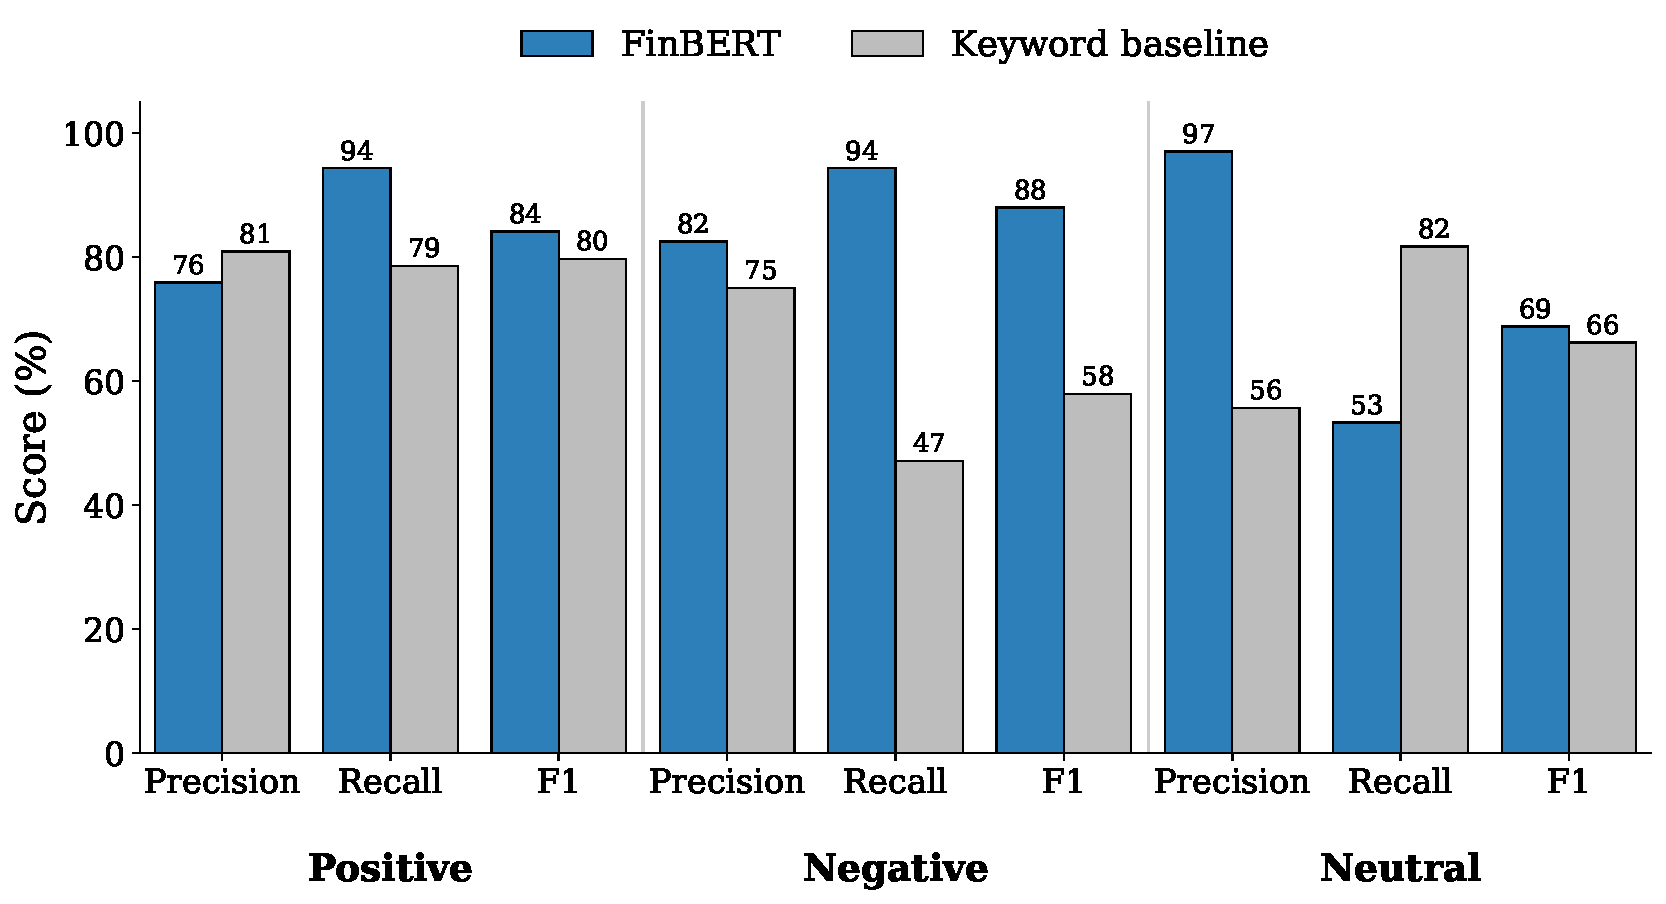
\includegraphics[width=\textwidth]{metrics_barchart.pdf}
%DIFDELCMD < %%%
%DIFDELCMD < \caption{%
{%DIFAUXCMD
\DIFdelFL{Per-class precision, recall and F1 for FinBERT (coloured blue bars) versus the
keyword baseline (grey bars) on the 200-sample benchmark. FinBERT's large recall
advantage on the negative class and the neutral asymmetry (high precision, low
recall) are immediately visible.}}
%DIFAUXCMD
%DIFDELCMD < \label{fig:bars}
%DIFDELCMD < \end{figure}
%DIFDELCMD < 

%DIFDELCMD < \begin{figure}[ht]
%DIFDELCMD < \centering
%DIFDELCMD < 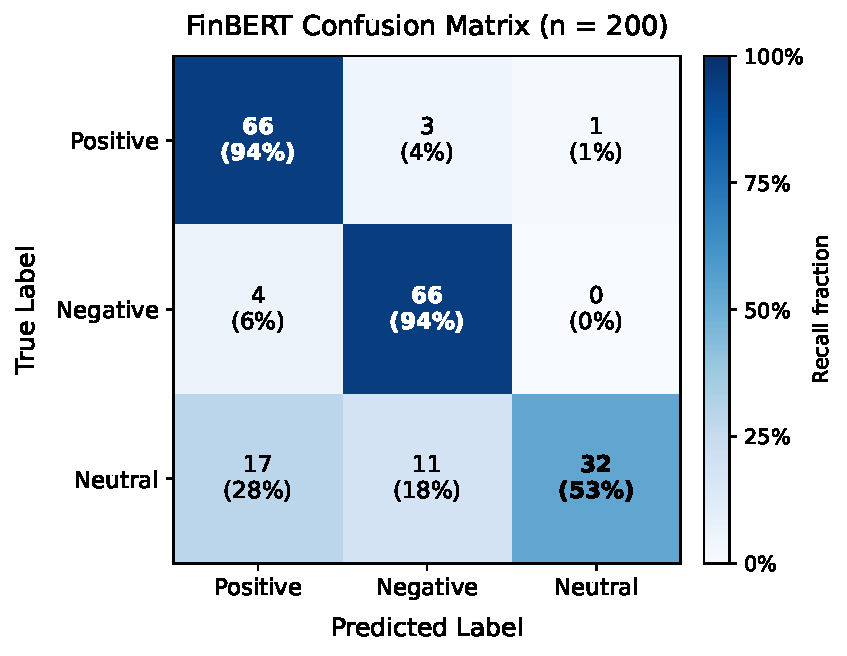
\includegraphics[width=0.6\textwidth]{confusion_matrix.pdf}
%DIFDELCMD < %%%
%DIFDELCMD < \caption{%
{%DIFAUXCMD
\DIFdelFL{Row-normalised confusion matrix for FinBERT on the 200-sample benchmark.
The strong diagonal on the positive and negative classes contrasts with the
dispersed neutral row, visualising the neutral recall deficit.}}
%DIFAUXCMD
%DIFDELCMD < \label{fig:cm}
%DIFDELCMD < \end{figure}
%DIFDELCMD < 

%DIFDELCMD < \subsection{Explainability-guided diagnosis}
%DIFDELCMD < %%%
\DIFdelend \DIFaddbegin \subsection{Explainability as hypothesis generation}
\DIFadd{LIME is used here to illustrate, not to establish, a candidate mechanism. The
positive and negative examples are drawn verbatim from the labelled evaluation set
of the deployed system (}\texttt{\DIFadd{labeled\_dataset.py}}\DIFadd{); the neutral example is a
variant of a neutral sentence in that set. Explanations use stock FinBERT with
5}{\DIFadd{,}}\DIFadd{000 perturbation samples, whitespace tokens and a fixed random state, and show
the eight highest-weighted tokens. }\DIFaddend Applied to unambiguous \DIFdelbegin \DIFdel{cases}\DIFdelend \DIFaddbegin \DIFadd{sentences}\DIFaddend , LIME assigns the
highest weights to semantically appropriate tokens\DIFdelbegin \DIFdel{(}\DIFdelend \DIFaddbegin \DIFadd{: }\DIFaddend ``surged'',
``\DIFdelbegin \DIFdel{raised'' , ``guidance}\DIFdelend \DIFaddbegin \DIFadd{significantly'' and ``raised}\DIFaddend '' for a positive prediction at \DIFdelbegin \DIFdel{95\% confidence
, }\DIFdelend \DIFaddbegin \DIFadd{95.0\% confidence
(}\DIFaddend Figure~\ref{fig:lime_pos}\DIFdelbegin \DIFdel{; ``decline'', ``sharp'' , ``missing}\DIFdelend \DIFaddbegin \DIFadd{), and ``layoffs'' and ``loss}\DIFaddend '' for a negative prediction
at \DIFdelbegin \DIFdel{97.6\% , }\DIFdelend \DIFaddbegin \DIFadd{96.9\% confidence (}\DIFaddend Figure~\ref{fig:lime_neg})\DIFdelbegin \DIFdel{, confirming the
explanations are meaningful rather than artefactual. The diagnostically decisive
case is a misclassified neutral sentence
: }\DIFdelend \DIFaddbegin \DIFadd{. For the neutral sentence
}\DIFaddend \emph{``The Federal Reserve kept interest rates unchanged, maintaining its cautious
outlook on inflation.''}\DIFaddbegin \DIFadd{, }\DIFaddend FinBERT predicts \emph{negative} (55.9\% confidence\DIFaddbegin \DIFadd{,
against 27.5\% for neutral}\DIFaddend ), and LIME \DIFdelbegin \DIFdel{identifies }\DIFdelend \DIFaddbegin \DIFadd{attributes this mainly to }\DIFaddend ``cautious'' and
``inflation''\DIFdelbegin \DIFdel{as the driving negative weights, both legitimate risk signals }\DIFdelend \DIFaddbegin \DIFadd{, followed by ``outlook'' and ``unchanged'', words that signal risk }\DIFaddend in
isolation but \DIFaddbegin \DIFadd{are }\DIFaddend contextually neutral here \DIFaddbegin \DIFadd{(Figure~\ref{fig:lime_neu})}\DIFaddend . This is \DIFdelbegin \DIFdel{precisely the
error pattern
visible in Table~\ref{tab:cm}: the model conflates neutral-framed risk vocabulary with genuine negative sentiment.
LIME thus converts an aggregate symptom (53.3\%
neutral recall) into a specific, lexically-localised mechanism, exactly the kind of actionable diagnosis that motivates atargeted intervention}\DIFdelend \DIFaddbegin \DIFadd{the
misclassified neutral example requested by Reviewer~2, and it shows the failure mode
directly: risk-laden vocabulary pulls a factual policy statement away from neutral.
These examples
suggested the hypothesis that exposure to neutral text containing sentiment-loaded
vocabulary would help more than exposure to neutral text in general. They are
single, hand-chosen explanations, and the hypothesis is tested directly by the
comparison of arms (a) and (b) below}\DIFaddend .

\begin{figure}[ht]
\centering
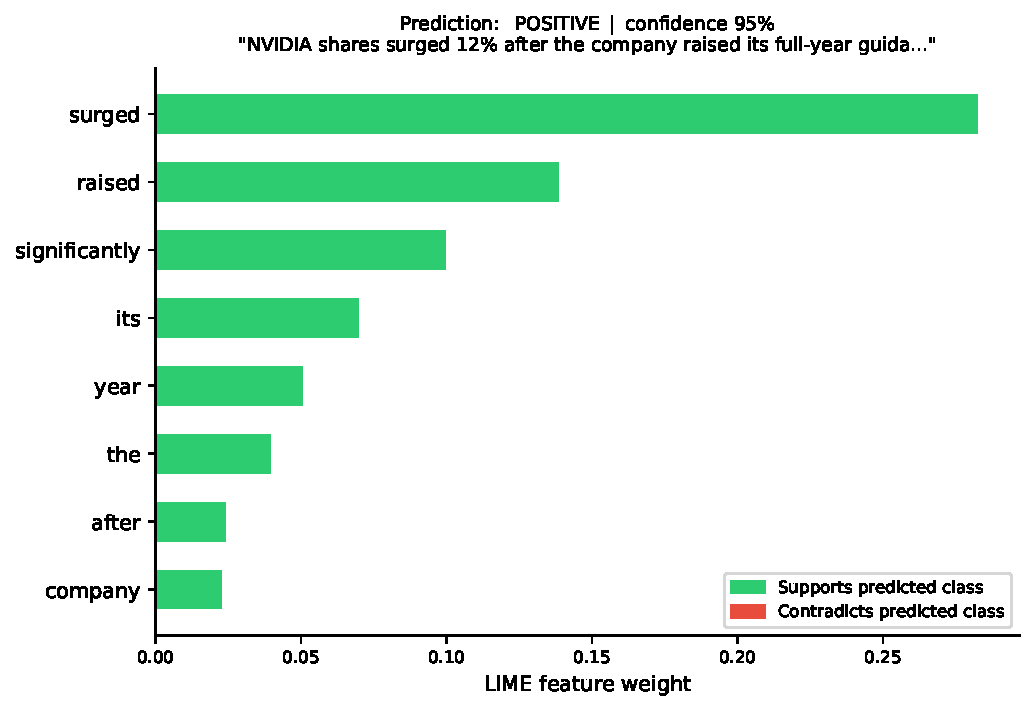
\includegraphics[width=\textwidth]{lime_positive.pdf}
\caption{LIME token weights for a positive financial sentence \DIFaddbeginFL \DIFaddFL{(illustrative)}\DIFaddendFL . Green
bars indicate tokens supporting the \emph{positive} prediction; red bars indicate
tokens pushing against it. \DIFaddbeginFL \DIFaddFL{Stock }\DIFaddendFL FinBERT predicted \emph{positive} at \DIFdelbeginFL \DIFdelFL{95}\DIFdelendFL \DIFaddbeginFL \DIFaddFL{95.0}\DIFaddendFL \%
confidence\DIFaddbeginFL \DIFaddFL{; }\emph{\DIFaddFL{surged}}\DIFaddFL{, }\emph{\DIFaddFL{significantly}} \DIFaddFL{and }\emph{\DIFaddFL{raised}} \DIFaddFL{carry the largest
weights}\DIFaddendFL .}
\label{fig:lime_pos}
\end{figure}

\begin{figure}[ht]
\centering
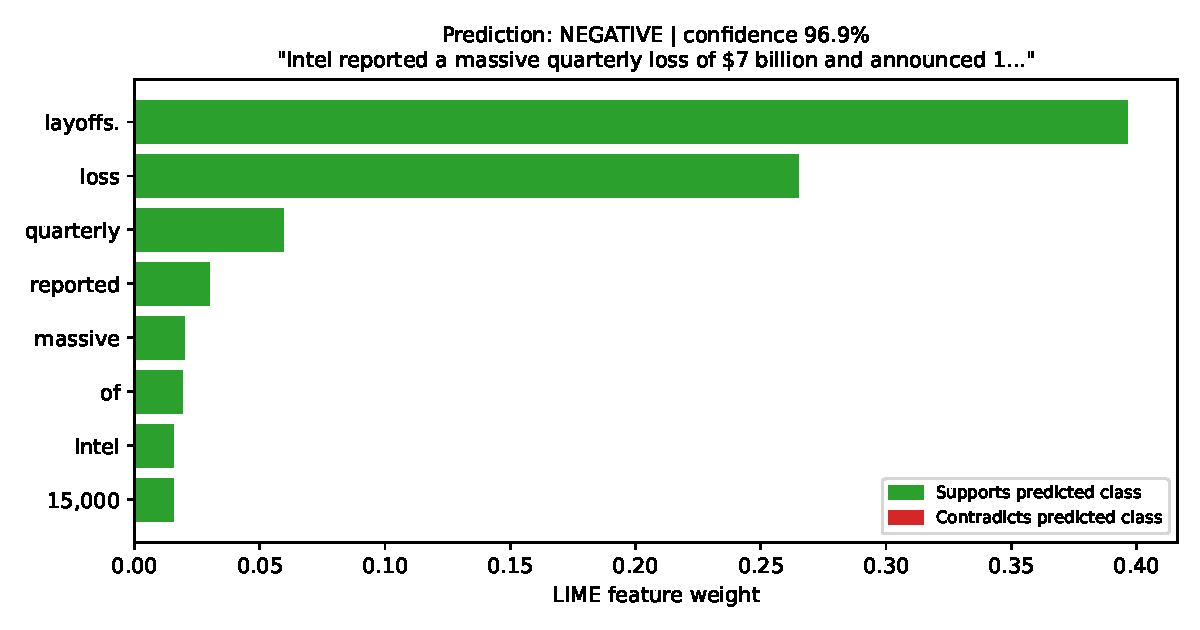
\includegraphics[width=\textwidth]{lime_negative.pdf}
\caption{LIME token weights for a negative financial sentence \DIFdelbeginFL \DIFdelFL{. }\DIFdelendFL \DIFaddbeginFL \DIFaddFL{(illustrative):
}\emph{\DIFaddFL{``Intel reported a massive quarterly loss of \$7 billion and announced 15,000
layoffs.''}} \DIFaddFL{Stock }\DIFaddendFL FinBERT predicted \emph{negative} at \DIFdelbeginFL \DIFdelFL{97.6}\DIFdelendFL \DIFaddbeginFL \DIFaddFL{96.9}\DIFaddendFL \% confidence;
\DIFdelbeginFL \emph{\DIFdelFL{decline}}%DIFAUXCMD
\DIFdelFL{, }\emph{\DIFdelFL{sharp}} %DIFAUXCMD
\DIFdelendFL \DIFaddbeginFL \emph{\DIFaddFL{layoffs}} \DIFaddendFL and \DIFdelbeginFL \emph{\DIFdelFL{missing}} %DIFAUXCMD
\DIFdelendFL \DIFaddbeginFL \emph{\DIFaddFL{loss}} \DIFaddendFL are the principal drivers.}
\label{fig:lime_neg}
\end{figure}

\DIFdelbegin %DIFDELCMD < \subsection{Targeted mitigation}
%DIFDELCMD < %%%
\DIFdel{Table~\ref{tab:finetune} reports the effect of }\DIFdelend \DIFaddbegin \begin{figure}[ht]
\centering
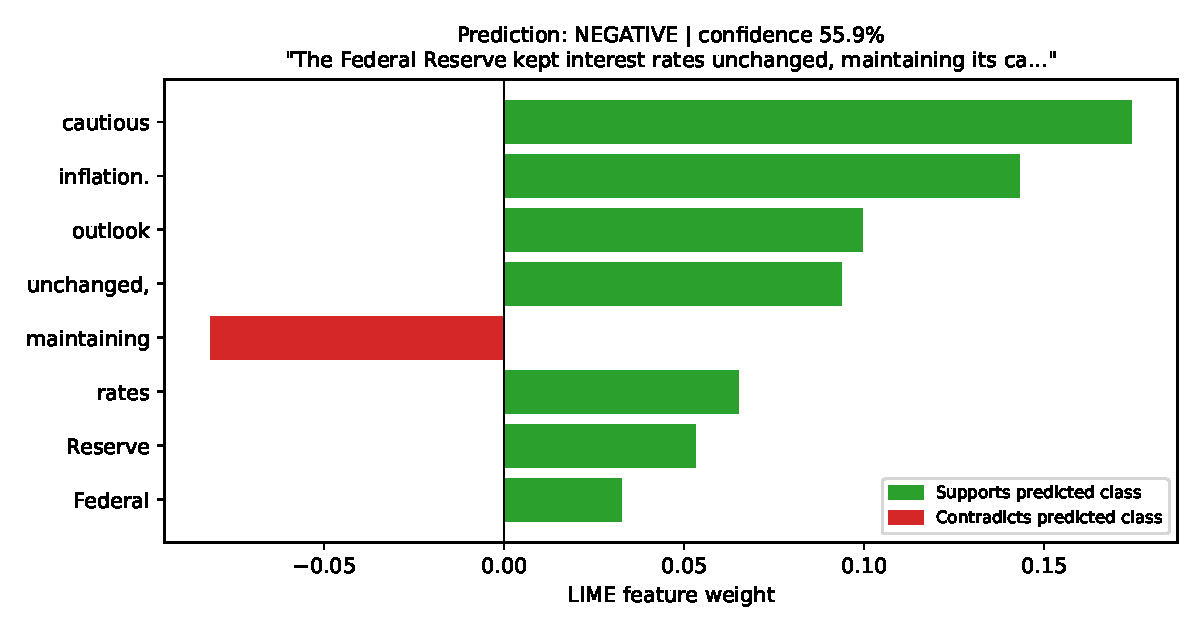
\includegraphics[width=\textwidth]{lime_neutral.pdf}
\caption{\DIFaddFL{LIME token weights for a gold-neutral financial sentence that stock FinBERT
misclassifies (illustrative). Stock FinBERT assigned 55.9\% probability to
}\emph{\DIFaddFL{negative}} \DIFaddFL{against 27.5\% to }\emph{\DIFaddFL{neutral}}\DIFaddFL{; }\emph{\DIFaddFL{cautious}} \DIFaddFL{and
}\emph{\DIFaddFL{inflation}} \DIFaddFL{are the top drivers towards the negative prediction.}}
\label{fig:lime_neu}
\end{figure}

\subsection{Fine-tuning arms on the benchmark}
\DIFadd{Table~\ref{tab:armres} summarises the 15 }\DIFaddend fine-tuning \DIFdelbegin \DIFdel{on the disjoint
300-sample neutral-loaded corpus, re-evaluated on the unchanged benchmark. Neutral
recall improves by 18.4 percentage points (53.3\%$\rightarrow$ 71.7\% )}\DIFdelend \DIFaddbegin \DIFadd{runs. All three arms raise
macro-F1 above stock FinBERT (49.8\%): to 59.1\% for the lexicon-loaded arm (a),
60.7\% for the random-neutral arm (b) and 53.4\% for the mixed arm (c), averaged over
five seeds. The gains come from the polarised classes. Every arm raises positive and
negative recall and lowers neutral recall from the stock 81.5\%, to 47.7\% (a), 60.6\%
(b) and 26.5\% (c), while neutral precision rises from 48.2\% to 63.1\%, 64.1\% and
76.8\% respectively. The arms predict neutral for 102.6 (a), 128.0 (b) and 46.8 (c)
items on average, against 135 gold neutral items and 228 for stock FinBERT. Arm (c)
is also the least stable across seeds (macro-F1 standard deviation 3.7 points).
The off-the-shelf Twitter-RoBERTa baseline (56.8\%) does not beat the two best
fine-tuned arms: it is 2.3 points below arm (a) and 3.9 points below arm (b), and 3.4
points above arm (c), but none of these differences is statistically distinguishable
(95\% CIs $[-8.8, +4.2]$, $[-10.1, +2.3]$ and $[-3.2, +10.1]$; Holm $p = 0.67$ for each;
Table~\ref{tab:boot}). Domain fine-tuning of FinBERT therefore matches, but is not
shown to exceed, a general social-media sentiment model.
}

\begin{table}[ht]
\centering
\caption{\DIFaddFL{Fine-tuned FinBERT on the 338-item benchmark: mean $\pm$ standard deviation
over five seeds, with 95\% $t$-intervals for macro-F1 and accuracy. Stock FinBERT
shown for reference, with the off-the-shelf Twitter-RoBERTa baseline (single
deterministic run).}}
\label{tab:armres}
\small
\begin{tabular}{lccccc}
\toprule
\textbf{Model} & \textbf{Macro-F1} & \textbf{Accuracy} & \textbf{Rec.\ pos.} & \textbf{Rec.\ neg.} & \textbf{Rec.\ neu.} \\
\midrule
Stock & 49.8\% & 53.0\% & 28.7\% & 42.0\% & 81.5\% \\
Twitter-RoBERTa & 56.8\% & 59.2\% & 45.1\% & 40.7\% & 83.0\% \\
(a) Lexicon-loaded & $59.1 \pm 0.9$ [58.0, 60.3] & $58.9 \pm 0.9$ [57.9, 60.0] & $63.3 \pm 2.3$ & $71.1 \pm 2.4$ & $47.7 \pm 4.0$ \\
(b) Random-neutral & $60.7 \pm 1.5$ [58.9, 62.6] & $60.8 \pm 1.5$ [59.0, 62.6] & $53.1 \pm 5.4$ & $72.8 \pm 1.5$ & $60.6 \pm 1.7$ \\
(c) Mixed & $53.4 \pm 3.7$ [48.8, 58.0] & $55.0 \pm 2.8$ [51.5, 58.5] & $68.4 \pm 7.2$ & $82.2 \pm 2.4$ & $26.5 \pm 9.0$ \\
\bottomrule
\end{tabular}
\end{table}

\DIFadd{Table~\ref{tab:boot} gives the paired comparisons. Against stock FinBERT, the
item-level bootstrap supports gains for arm (a) ($+9.3$ points of macro-F1}\DIFaddend , \DIFdelbegin \DIFdel{the precise
effect the diagnosis predicted; neutral precision falls modestly (97.0\%
$\rightarrow$ 91.8\% )}\DIFdelend \DIFaddbegin \DIFadd{95\% CI
$[+3.7, +15.1]$}\DIFaddend , \DIFdelbegin \DIFdel{as expected when the model is encouraged to predict neutral
more often, but neutral F1 nonetheless rises by 11.7 points. Overall accuracy
increases to 86.5\%and macro F1 to 85.2\% }\DIFdelend \DIFaddbegin \DIFadd{Holm-adjusted $p = 0.004$) and arm (b) ($+11.0$ points,
$[+5.6, +16.5]$}\DIFaddend , \DIFdelbegin \DIFdel{and polarised-class F1 is preserved (both
within 0.5 points of the stock model) }\DIFdelend \DIFaddbegin \DIFadd{Holm-adjusted $p < 0.001$), but not for arm (c) ($+3.6$ points,
$[-2.6, +10.0]$}\DIFaddend , \DIFdelbegin \DIFdel{confirming the intervention does not
simply
trade one class error for another. The diagnosed failure mode is therefore
demonstrably addressable with asmall, targeted dataset}\DIFdelend \DIFaddbegin \DIFadd{Holm-adjusted $p = 0.51$). The central comparison for the LIME
hypothesis, lexicon-loaded versus random neutrals, shows no advantage for lexical
targeting: arm (a) is 1.6 points }\emph{\DIFadd{below}} \DIFadd{arm (b) ($[-5.0, +1.7]$,
Holm-adjusted $p = 0.51$; seed-paired $t$-test $p = 0.20$, Wilcoxon $p = 0.31$). Both
neutral arms outperform the mixed arm in the bootstrap (Holm-adjusted $p = 0.012$
for (a) and $0.004$ for (b)); the seed-paired tests point the same way but do not
survive correction (Holm-adjusted $t$-test $p = 0.072$ for both; Wilcoxon $p = 0.0625$
before correction, the minimum attainable with five seeds). At the level of single
runs, exact McNemar tests against stock reach uncorrected $p < 0.05$ in all five arm
(b) runs and one arm (a) run, and in no arm (c) run; after Holm correction across the
15 runs only one (arm (b), seed 21; adjusted $p = 0.019$) remains below 0.05. Gains
are thus clearer when seeds are pooled than for any individual run.
}

\begin{table}[ht]
\centering
\caption{\DIFaddFL{Item-level paired bootstrap of seed-averaged macro-F1 on the benchmark
($B = 10{,}000$; differences in percentage points; Holm correction over the six
comparisons in the upper block; the Twitter-RoBERTa comparisons in the lower block
form a separate family of four).}}
\label{tab:boot}
\begin{tabular}{lccc}
\toprule
\textbf{Comparison} & \textbf{Difference} & \textbf{95\% CI} & \textbf{Holm $p$} \\
\midrule
(a) vs stock & $+9.3$ & $[+3.7, +15.1]$ & 0.004 \\
(b) vs stock & $+11.0$ & $[+5.6, +16.5]$ & $<0.001$ \\
(c) vs stock & $+3.6$ & $[-2.6, +10.0]$ & 0.514 \\
(a) vs (b) & $-1.6$ & $[-5.0, +1.7]$ & 0.514 \\
(a) vs (c) & $+5.7$ & $[+2.0, +9.6]$ & 0.012 \\
(b) vs (c) & $+7.4$ & $[+3.5, +11.4]$ & 0.004 \\
\midrule
Twitter-RoBERTa vs stock & $+7.0$ & $[+0.1, +14.0]$ & 0.190 \\
Twitter-RoBERTa vs (a) & $-2.3$ & $[-8.8, +4.2]$ & 0.672 \\
Twitter-RoBERTa vs (b) & $-3.9$ & $[-10.1, +2.3]$ & 0.672 \\
Twitter-RoBERTa vs (c) & $+3.4$ & $[-3.2, +10.1]$ & 0.672 \\
\bottomrule
\end{tabular}
\end{table}

\DIFadd{Table~\ref{tab:source} breaks the benchmark down by channel. The channels differ
in class mix (news is 57\% neutral, Twitter 24\%) and in ticker concentration (the
five most frequent tickers cover 48\% of news items but 24\% of Twitter items).
Stock FinBERT and the keyword baseline are strongest on news and weakest on Twitter,
and the fine-tuning gains are concentrated on Twitter, where arms (a) and (b) reach
63.5\% and 63.3\% macro-F1 against 39.9\% for stock; on news only arm (b) exceeds
stock, and on Reddit no system exceeds 52\%. Each channel has only 108--115 items,
with 17 to 29 items in the smallest class, so these per-channel figures are
descriptive and were not tested for significance}\DIFaddend .

\begin{table}[ht]
\centering
\caption{\DIFdelbeginFL \DIFdelFL{Stock FinBERT versus neutral-focused fine-tuned FinBERT on }\DIFdelendFL \DIFaddbeginFL \DIFaddFL{Benchmark composition and macro-F1 (\%) by channel. Arms are means over five
seeds. Tickers are }\DIFaddendFL the \DIFdelbeginFL \DIFdelFL{200-sample
benchmark}\DIFdelendFL \DIFaddbeginFL \DIFaddFL{stored ticker tag; every item has one. Per-channel macro-F1 is
descriptive only (small $n$, no significance tests)}\DIFaddendFL .}
\DIFdelbeginFL %DIFDELCMD < \label{tab:finetune}
%DIFDELCMD < \begin{tabular}{lccccc}
%DIFDELCMD < \toprule
%DIFDELCMD < \textbf{Model} & \textbf{Accuracy} & \textbf{Macro F1} & \textbf{Neu.\ prec.} & \textbf{Neu.\ recall} & \textbf{Neu.\ F1} \\
%DIFDELCMD < \midrule
%DIFDELCMD < FinBERT (stock)      & 82.0\% & 80.3\% & \textbf{97.0\%} & 53.3\% & 68.8\% \\
%DIFDELCMD < FinBERT (fine-tuned) & \textbf{86.5\%} & \textbf{85.2\%} & 91.8\% & \textbf{71.7\%} & \textbf{80.5\%} \\
%DIFDELCMD < \midrule
%DIFDELCMD < \textit{Delta} & \textit{+4.5 pp} & \textit{+4.9 pp} & \textit{$-$5.2 pp} & \textit{+18.4 pp} & \textit{+11.7 pp} \\
%DIFDELCMD < \bottomrule
%DIFDELCMD < \end{tabular}
%DIFDELCMD < %%%
\DIFdelendFL \DIFaddbeginFL \label{tab:source}
\small
\begin{tabular}{lcccc}
\toprule
 & \textbf{News} & \textbf{Reddit} & \textbf{Twitter} & \textbf{All} \\
\midrule
Items (pos / neg / neu) & 32 / 17 / 66 & 38 / 29 / 41 & 52 / 35 / 28 & 122 / 81 / 135 \\
Post dates & 2017-08 -- 2026-07 & 2021-02 -- 2026-08 & 2022-01 -- 2026-04 & 2017-08 -- 2026-08 \\
Distinct tickers & 49 & 47 & 79 & 152 \\
Top-5 ticker share & 47.8\% & 38.0\% & 24.3\% & 20.1\% \\
\midrule
Stock FinBERT & 67.7 & 42.4 & 39.9 & 49.8 \\
(a) Lexicon-loaded & 60.8 & 48.6 & 63.5 & 59.1 \\
(b) Random-neutral & 70.7 & 43.8 & 63.3 & 60.7 \\
(c) Mixed & 57.0 & 46.2 & 48.1 & 53.4 \\
Twitter-RoBERTa & 62.4 & 51.7 & 51.4 & 56.8 \\
Keyword baseline & 64.3 & 40.2 & 35.5 & 46.7 \\
\bottomrule
\end{tabular}
\DIFaddendFL \end{table}

\DIFdelbegin \DIFdel{We are explicit about the strength of this evidence: the $+4.5$-point accuracy gain
is from a single 200-sample benchmark and a single fine-tuning seed, without
cross-validation,
}\DIFdelend \DIFaddbegin \DIFadd{Table~\ref{tab:neuerr} aggregates the errors that involve the neutral class.
Stock FinBERT and Twitter-RoBERTa err mainly by absorbing polar items into neutral
(118 }\DIFaddend and \DIFdelbegin \DIFdel{the }\DIFdelend \DIFaddbegin \DIFadd{102 such errors), and their few errors on gold-neutral items lean slightly
negative (15 vs 10 and 14 vs 9). Fine-tuning reverses the direction: errors into
neutral fall to 38.2 (a), 46.2 (b) and 11.0 (c), while gold-neutral items are pushed
out of neutral, mostly towards positive for arms (a) and (c) (45.4 and 59.6 items)
and about equally in both directions for arm (b) (27.0 negative, 26.2 positive).
}

\begin{table}[ht]
\centering
\caption{\DIFaddFL{Neutral-related error counts on the benchmark (135 gold-neutral, 122
positive, 81 negative items). Arms are means over five seeds.}}
\label{tab:neuerr}
\small
\begin{tabular}{lcccccc}
\toprule
 & \multicolumn{3}{c}{\textbf{Gold neutral predicted as}} & \multicolumn{2}{c}{\textbf{Into neutral}} & \\
\cmidrule(lr){2-4}\cmidrule(lr){5-6}
\textbf{Model} & \textbf{neu} & \textbf{neg} & \textbf{pos} & \textbf{pos$\to$neu} & \textbf{neg$\to$neu} & \textbf{pos$\leftrightarrow$neg} \\
\midrule
Stock FinBERT & 110 & 15 & 10 & 74 & 44 & 16 \\
(a) Lexicon-loaded & 64.4 & 25.2 & 45.4 & 24.0 & 14.2 & 30.0 \\
(b) Random-neutral & 81.8 & 27.0 & 26.2 & 32.2 & 14.0 & 33.0 \\
(c) Mixed & 35.8 & 39.6 & 59.6 & 8.0 & 3.0 & 42.0 \\
Twitter-RoBERTa & 112 & 14 & 9 & 61 & 41 & 13 \\
Keyword baseline & 91 & 25 & 19 & 64 & 34 & 31 \\
\bottomrule
\end{tabular}
\end{table}

\subsection{Out-of-domain checks}
\DIFadd{Table~\ref{tab:ood} reports the out-of-domain evaluations. On both external datasets
the }\DIFaddend fine-tuned \DIFdelbegin \DIFdel{model has not been stress-tested on }\DIFdelend \DIFaddbegin \DIFadd{models score below stock FinBERT. On the Twitter Financial News
validation split, macro-F1 falls from 66.8\% (stock) to 57.2\% for arm (a)
($-9.6$ points, bootstrap 95\% CI $[-11.5, -7.7]$), 63.0\% for arm (b) ($-3.8$,
$[-5.5, -2.1]$) and 39.7\% for arm (c) ($-27.1$, $[-29.2, -25.0]$). On Financial
PhraseBank, where stock FinBERT's scores are in-sample, }\DIFaddend the \DIFdelbegin \DIFdel{full
live distribution.
The result is reported as an indicative demonstration of the diagnosis-to-mitigation loop, not as adefinitive performance claim
(Section~\ref{sec:discussion}) ; a multi-seed cross-validated protocol is
provided as
reproducible code (Section~\ref{sec:reprod})}\DIFdelend \DIFaddbegin \DIFadd{fine-tuned models also
fall below stock on both subsets, with the same ordering ((b) above (a) above (c)).
In each case the fall is concentrated in the neutral class: on Twitter Financial
News, where 1}{\DIFadd{,}}\DIFadd{566 of 2}{\DIFadd{,}}\DIFadd{388 items are neutral, stock FinBERT predicts neutral for
1}{\DIFadd{,}}\DIFadd{388 items, against 747 (a), 1}{\DIFadd{,}}\DIFadd{019 (b) and 215 (c) for the fine-tuned models,
and neutral recall falls from 75.6\% to 44.3\%, 59.4\% and 13.2\%.
}

\begin{table}[ht]
\centering
\caption{\DIFaddFL{Out-of-domain evaluation (macro-F1 / accuracy; neutral recall in
parentheses). One seed per arm, chosen by validation macro-F1. Stock FinBERT was
fine-tuned on Financial PhraseBank, so its PhraseBank scores are in-sample.}}
\label{tab:ood}
\small
\begin{tabular}{lccc}
\toprule
\textbf{Model} & \textbf{PhraseBank all-agree} & \textbf{PhraseBank 50\%-agree} & \textbf{Twitter Fin.\ News (val.)} \\
 & ($n = 2{,}264$) & ($n = 4{,}846$) & ($n = 2{,}388$) \\
\midrule
Stock & 96.3 / 97.2 (96.7) & 88.3 / 89.0 (85.8) & 66.8 / 72.5 (75.6) \\
(a) seed 84 & 92.0 / 93.5 (91.8) & 82.0 / 82.2 (74.0) & 57.2 / 57.8 (44.3) \\
(b) seed 84 & 93.3 / 94.9 (94.4) & 84.4 / 85.5 (80.4) & 63.0 / 65.8 (59.4) \\
(c) seed 21 & 77.9 / 76.8 (64.4) & 67.1 / 64.6 (42.9) & 39.7 / 38.6 (13.2) \\
\bottomrule
\end{tabular}
\end{table}

\paragraph{Domain shift.} \DIFadd{Taken together, the in-domain and out-of-domain results
indicate that fine-tuning adapts FinBERT to the class balance and labelling
conventions of the target data rather than repairing a general weakness. On the
project's multi-source benchmark, where stock FinBERT over-predicts neutral, the
arms shift predictions toward the polarised classes and seed-averaged macro-F1
rises by 9 to 11 points for the two neutral arms. On Financial PhraseBank and Twitter Financial News, whose texts are
predominantly professionally written or headline-style and whose neutral class is
large, the same shift away from neutral lowers neutral recall and overall
performance below stock FinBERT. The mixed arm (c), which adds polarised examples
rather than neutrals, shifts furthest and transfers worst. Gains on an in-domain
benchmark should therefore not be read as evidence of better financial sentiment
classification in general; whether a given adaptation helps depends on how closely
the deployment distribution and label definitions match the fine-tuning data}\DIFaddend .

\subsection{Supporting analyses}
\paragraph{Sentiment-price correlation.}
A demonstrative run of the correlation engine across a nine-ticker panel (90-day
window, same-day alignment) produced modest, heterogeneous, and mostly
non-significant effects. Same-day Pearson coefficients ranged from $r = -0.10$ (SPY)
to $+0.24$ (NVDA); NVDA, AAPL and AMZN were individually significant at
$\alpha = 0.05$ (uncorrected), but under a Bonferroni correction for nine tickers
($\alpha_B = 0.0056$) none reached significance, and no Granger test attained
$p < 0.05$ at one- or two-day lags. SPY's near-zero coefficient is the expected null
for a diversified index tracker. These magnitudes are consistent with the literature
that sentiment-return effects are statistically detectable but economically small
\citep{tetlock2007,kraaijeveld2020}, and the rolling-correlation standard deviations
(0.14 to 0.34) show the relationship is unstable across sub-windows. We report this
as an honest null or modest result rather than selecting favourable windows.

\paragraph{Finance-emotion enrichment.}
Because no public benchmark annotates financial text at this emotion granularity, an
accuracy evaluation is not possible; we instead ran a component-contribution
ablation measuring how often removing a component flips the dominant emotion label on
the \DIFdelbegin \DIFdel{200-sample benchmark. The domain lexicon is load-bearing }\DIFdelend \DIFaddbegin \DIFadd{frozen 338-item benchmark, with FinBERT class probabilities supplied to the
taxonomy. Zeroing the entropy term changes 36.1\% of labels (122/338), whereas
removing the domain lexicon changes 2.1\% }\DIFaddend (\DIFdelbegin \DIFdel{16.0\% of labels change
when it is removed; all samples collapse to ``mixed'' ), whereas zeroing the entropy
term flips no
labels, an honest negative finding indicating the entropy componentrequires re-tuning. The }\DIFdelend \DIFaddbegin \DIFadd{7/338). Under the full configuration the
labels are dominated by ``uncertainty'' (250/338). An earlier version of this ablation
did not pass the class probabilities to the taxonomy; this has been corrected. Because no
emotion ground truth is available, these figures measure each component's influence,
not its accuracy, and the }\DIFaddend enrichment layer is therefore reported as deployed but only
partially validated.

\paragraph{System performance.}
FinBERT batch inference required \DIFdelbegin \DIFdel{2.15}\DIFdelend \DIFaddbegin \DIFadd{7.7}\DIFaddend ~s for \DIFdelbegin \DIFdel{200 samples }\DIFdelend \DIFaddbegin \DIFadd{the 338 benchmark items }\DIFaddend ($\approx$\DIFdelbegin \DIFdel{11}\DIFdelend \DIFaddbegin \DIFadd{23}\DIFaddend ~ms per
text\DIFaddbegin \DIFadd{; median of five runs, batch size 32, 8-thread CPU, no GPU}\DIFaddend );
the keyword baseline was effectively instantaneous \DIFaddbegin \DIFadd{($<$5~ms for all 338 items)}\DIFaddend ; LIME explanations took 15 to
40~s, consistent with an on-demand rather than bulk feature.

% =====================================================================
\section{Discussion}\label{sec:discussion}
% =====================================================================
\subsection{Interpretation and significance}
\DIFdelbegin \DIFdel{The principal finding is that FinBERT's
}\DIFdelend \DIFaddbegin \DIFadd{Three findings stand out. First, on a benchmark sampled from the deployed system's
own multi-source data, stock FinBERT does not show the neutral-recall deficit
reported on curated news text; it over-predicts neutral (228 predictions against 135
gold items), and its main errors are polarised posts labelled neutral. The
direction of FinBERT's }\DIFaddend neutral-class \DIFdelbegin \DIFdel{deficit, usually reported as
an inert number, is a }\emph{\DIFdel{specific and repairable}} %DIFAUXCMD
\DIFdel{failure mode. The
conservatism
that produces 97.0\% neutral precision at 53.3\% recall is, in one sense, defensible
for a financial dashboard: mislabelling a strongly positive announcement as neutral is arguably worse for a user than the reverse.
But the 28/60 neutral error rate is a
non-trivial source of label noise, particularly for factual news.
The contribution
of this paper is to show }\emph{\DIFdel{why}} %DIFAUXCMD
\DIFdel{the errors occur and }\emph{\DIFdel{that}} %DIFAUXCMD
\DIFdel{they can be
reduced: LIME localises the cause to neutral-framed risk vocabulary, and }\DIFdelend \DIFaddbegin \DIFadd{error therefore depends on the text
distribution and the label definitions, and a single benchmark is not enough to
characterise it.
}

\DIFadd{Second, }\DIFaddend fine-tuning on a \DIFdelbegin \DIFdel{small corpus of exactly that kind of text recovers 18.4 points of recall without
collateral damage to the
polarised classes. This is a concrete instance of XAI used
}\DIFdelend \DIFaddbegin \DIFadd{modest amount of in-domain labelled data improves in-domain
performance: both neutral arms raise seed-averaged macro-F1 by roughly 9 to 11
points, and the gains survive an item-level paired bootstrap with Holm correction.
The improvement comes from the polarised classes, at the cost of neutral recall.
}

\DIFadd{Third, the LIME-motivated selection of lexicon-loaded neutrals gave no advantage over
randomly chosen neutrals; if anything, the random-neutral arm scored slightly higher
and transferred better out of domain. The LIME examples remain useful for
illustrating how individual risk words can shift a prediction, but in this study
they did not identify a data-selection strategy that outperformed a random control.
We therefore present LIME as hypothesis-generating rather than as the source of the
improvement. More broadly, the results illustrate the value of testing an
explanation-derived hypothesis against a matched control, rather than reporting the
intervention alone; this is the use of XAI }\DIFaddend as a diagnostic feedback mechanism \DIFdelbegin \DIFdel{rather than a presentation layer, the use case
}\DIFdelend that
surveys identify as under-explored \citep{yeo2025}\DIFaddbegin \DIFadd{, including when the feedback is
negative}\DIFaddend .

\DIFdelbegin \DIFdel{A second, methodological contribution is the
demonstration that applied
financial-sentiment comparisons can and
should be made with paired significance
testing. A 13.5-point accuracy gap is only a defensible claim once a McNemar test
($p = 0.002$) and non-overlapping bootstrap intervals rule out sampling variation;
many comparable studies report point estimates alone}\DIFdelend \DIFaddbegin \DIFadd{The out-of-domain results qualify the in-domain gains. All fine-tuned models score
below stock FinBERT on Financial PhraseBank and on Twitter Financial News, with the
largest drops for the mixed arm. Adaptation to one distribution's class balance and
labelling conventions carries a cost elsewhere, so in-domain gains should be
reported together with out-of-domain checks}\DIFaddend .

\subsection{Threats to validity and limitations}
We state limitations plainly. (i)~\emph{\DIFdelbegin \DIFdel{Benchmark scale and annotation}\DIFdelend \DIFaddbegin \DIFadd{Label provenance}\DIFaddend .} \DIFdelbegin \DIFdel{The
benchmark is 200 samples, labelled by a single author(D.H. ), validated by an LLM cross-pass and a single human annotator on a 100-sample subset; this is stronger than
single-annotator labelling but not equivalent to }\DIFdelend \DIFaddbegin \DIFadd{Benchmark and training
labels were produced by model-assisted labelling under a written rubric, with human
audit by one author. Audit agreement was substantial \mbox{%DIFAUXCMD
\citep{landis1977} }\hskip0pt%DIFAUXCMD
($\kappa = 0.807$ on 31
held-out reserve items) and neutral precision in the training pool was 23/29 on a 30-item blind
check, but these audits are small and the labels are not }\DIFaddend a multi-annotator
\DIFdelbegin \DIFdel{panel of the kind
used to build Financial PhraseBank. Scaling the benchmark to several thousand samples
and commissioning a panel are priority future work}\DIFdelend \DIFaddbegin \DIFadd{consensus. Systematic labelling conventions are shared by the benchmark and the
training arms, which may inflate in-domain gains relative to independently labelled
data}\DIFaddend . (ii)~\emph{\DIFdelbegin \DIFdel{Strength of the
mitigation evidence}\DIFdelend \DIFaddbegin \DIFadd{Benchmark composition}\DIFaddend .} The \DIFdelbegin \DIFdel{fine-tuning result rests on }\DIFdelend \DIFaddbegin \DIFadd{338-item benchmark is mostly a
channel-stratified random sample, but includes a negative-lexicon top-up (56 items)
and is modest in size. (iii)~}\emph{\DIFadd{Statistical power.}} \DIFadd{Five seeds per arm give low
power for seed-level tests (the exact Wilcoxon test cannot reach $p < 0.0625$), and
seed-paired arm comparisons do not survive Holm correction; item-level tests pool
seeds and should be read with that in mind. (iv)~}\emph{\DIFadd{Out-of-domain evidence.}} \DIFadd{The
out-of-domain evaluations use }\DIFaddend a single seed \DIFdelbegin \DIFdel{and a single
benchmark without cross-validation, and }\DIFdelend \DIFaddbegin \DIFadd{per arm, chosen by validation macro-F1,
so they do not capture seed variance; stock FinBERT's PhraseBank scores are
in-sample. (v)~}\emph{\DIFadd{Arm design.}} \DIFadd{Arms (a) and (b) share a 600-item
positive/negative base, a deviation from the planned neutral-only arms made after a
pilot collapsed to all-neutral predictions; arm (c) consequently differs in class
proportions, so its contrast with the other arms mixes class prior with data type.
(vi)~}\emph{\DIFadd{Lost original data.}} \DIFadd{The fine-tuning corpus and run behind the earlier
version of this study could not be recovered, and the original 200-item benchmark
is not used; }\DIFaddend the \DIFdelbegin \DIFdel{fine-tuned model has not been deployed or
evaluated on the full multi-source distribution; it evidences the diagnosis-to-mitigation loop but is not a definitive performance claim.
(iii}\DIFdelend \DIFaddbegin \DIFadd{earlier fine-tuning result is superseded, not replicated.
(vii}\DIFaddend )~\emph{LIME stability.} LIME explanations are local linear approximations\DIFdelbegin \DIFdel{and
}\DIFdelend \DIFaddbegin \DIFadd{, }\DIFaddend can
vary across runs \DIFdelbegin \DIFdel{; they are corroborating evidence, not guarantees, }\DIFdelend and can in principle be adversarially fooled \citep{slack2020}\DIFdelbegin \DIFdel{. (iv}\DIFdelend \DIFaddbegin \DIFadd{;
the examples shown are illustrative. (viii}\DIFaddend )~\emph{Data imbalance.} The
Twitter subcorpus is smaller and shallower than the Reddit and news subcorpora
because of X API v2 quota constraints, so Twitter is a secondary signal and
Twitter-only views carry lower statistical power. (\DIFdelbegin \DIFdel{v}\DIFdelend \DIFaddbegin \DIFadd{ix}\DIFaddend )~\emph{Correlation is not
causation.} The correlation engine is an exploratory tool; short-window sentiment
series are noisy and non-stationary, macro events confound sentiment and price
simultaneously, and the post-2008 liquidity regime weakens fundamental-to-price
linkages. The reported null Granger results should be read accordingly.
(\DIFdelbegin \DIFdel{vi}\DIFdelend \DIFaddbegin \DIFadd{x}\DIFaddend )~\emph{Enrichment validation.} The finance-emotion layer is deployed but lacks an
accuracy evaluation against an annotated emotion corpus, which does not yet exist for
these classes.

\subsection{Ethical considerations}
All data are publicly available and anonymised at ingestion, in line with platform
terms of service and the institutional ethical framework. Two broader issues warrant
note. First, a sentiment-analytics tool confers an informational advantage on its
users, connecting to long-standing debates on market efficiency \citep{fama1970}.
Second, where natural-language summaries of sentiment are generated, model outputs
can present statistical artefacts as confident narratives; outputs should therefore
be accompanied by explicit documentation of intended use and limitations, an approach
consistent with the model-cards framework \citep{mitchell2019}. This study is for
academic purposes; commercial deployment would require additional governance.

% =====================================================================
\section{Conclusions}\label{sec:conclusion}
% =====================================================================
\DIFdelbegin \DIFdel{A model error you cannot explain is a model error you cannot fix. This paper turned
}\DIFdelend \DIFaddbegin \DIFadd{This paper set out to explain and reduce }\DIFaddend FinBERT's \DIFdelbegin \DIFdel{familiar }\DIFdelend neutral-class \DIFdelbegin \DIFdel{weakness into a diagnosable and repairable failure
mode, and demonstrated an explainability-guided loop that closes the gap between
spotting a model error and repairing it}\DIFdelend \DIFaddbegin \DIFadd{error on
multi-source investor text, and to test whether a LIME-derived hypothesis could guide
the choice of fine-tuning data}\DIFaddend . On a \DIFdelbegin \DIFdel{purpose-built multi-source benchmark , FinBERT significantly
outperformed a finance-lexicon baseline (82.0\%vs 68.5\%accuracy; McNemar
$p = 0.002$) , but its 53.3\% neutral recall was traced by LIME to a single mechanism:
contextually neutral risk vocabulary attributed to the negative class.
A targeted
fine-tuning intervention on a small, disjoint corpus of neutral-but-lexically-loaded
text recovered neutral recallby 18.4 points and lifted accuracy to 86.5\% while
preserving polarised-class performance.
The methodological message generalises beyond
FinBERT: local interpretability can be used as an instrument to localise systematic
errors precisely enough to motivate proportionate, measurable mitigations, and applied sentiment comparisons should be reported with paired significance testing}\DIFdelend \DIFaddbegin \DIFadd{338-item benchmark drawn from the deployed
system's database, stock FinBERT over-predicted neutral (neutral recall 81.5\%,
precision 48.2\%) rather than under-predicting it. Fine-tuning on 900-item arms that
share a positive/negative base raised seed-averaged macro-F1 from 49.8\% to 59.1\%
(lexicon-loaded neutrals) and 60.7\% (random neutrals), with gains supported by a
paired item-level bootstrap after Holm correction; a mixed arm gave no reliable gain.
Selecting neutrals by the sentiment-loaded vocabulary that LIME highlighted gave no
advantage over a random-neutral control. On two out-of-domain datasets, every
fine-tuned model scored below stock FinBERT, mainly through lower neutral recall.
The evidence therefore supports in-domain adaptation with an out-of-domain cost, not
a general repair, and it shows the value of testing explanation-derived hypotheses
against matched controls and reporting paired significance tests}\DIFaddend .

Future work follows directly from the limitations. The most valuable next steps are
(i)~\DIFdelbegin \DIFdel{scaling }\DIFdelend \DIFaddbegin \DIFadd{independent multi-annotator labelling of }\DIFaddend the benchmark and \DIFdelbegin \DIFdel{commissioning a multi-annotator panel}\DIFdelend \DIFaddbegin \DIFadd{training data}\DIFaddend ;
(ii)~\DIFdelbegin \DIFdel{validating
the fine-tuning result under cross-validation and on the full live distribution}\DIFdelend \DIFaddbegin \DIFadd{multi-seed out-of-domain evaluation and adaptation methods that limit
out-of-domain loss}\DIFaddend ; (iii)~\DIFaddbegin \DIFadd{extending the baseline comparison beyond the
keyword lexicon and Twitter-RoBERTa to current financial LLMs \mbox{%DIFAUXCMD
\citep{wu2023,fatouros2023}}\hskip0pt%DIFAUXCMD
; (iv)~}\DIFaddend constructing
an annotated financial-emotion corpus to evaluate the enrichment layer formally; \DIFdelbegin \DIFdel{(iv)~extending the baseline comparison to current financial LLMs
\mbox{%DIFAUXCMD
\citep{wu2023,fatouros2023}}\hskip0pt%DIFAUXCMD
; }\DIFdelend and
(v)~feeding the resulting multi-source sentiment signal into hybrid temporal graph
models for price prediction \citep{lynch2025}.
\DIFdelbegin \DIFdel{Each builds
on the infrastructure and benchmark established here.
}\DIFdelend 

\paragraph{Reproducibility.}\label{sec:reprod}
The \DIFdelbegin \DIFdel{evaluation harness, the paired-significance and bootstrap routines, a multi-seed
cross-validated }\DIFdelend \DIFaddbegin \DIFadd{analysis code is available from the authors on reasonable request (see the Data
availability statement). It comprises the benchmark sampling scripts and the frozen 338-item
benchmark with its labels; the build script and manifests for the three 900-item
training arms; the }\DIFaddend fine-tuning \DIFdelbegin \DIFdel{protocol, }\DIFdelend \DIFaddbegin \DIFadd{runner and batch driver used for the 15 runs (three
arms $\times$ five seeds, 13, 21, 42, 84 }\DIFaddend and \DIFdelbegin \DIFdel{an external Financial PhraseBank comparison are released as runnable code accompanying this submission (see the Data
availability statement}\DIFdelend \DIFaddbegin \DIFadd{168), whose per-run outputs record the
selected epoch, validation and benchmark metrics and per-item benchmark predictions
and logits for every epoch; the statistics script (exact McNemar tests, item-level
paired bootstrap with $B = 10{,}000$ and fixed seed 20261024, seed-paired tests and
Holm correction) with its outputs; the Financial PhraseBank and Twitter Financial
News evaluation scripts and outputs; the keyword-baseline run on the benchmark; and a
locked list of CPU package versions. Model checkpoints are saved for the three
retrained models used in the out-of-domain evaluations (arms (a) and (b), seed 84;
arm (c), seed 21), which reproduced their original benchmark predictions exactly;
checkpoints for the remaining runs were not retained. Also included are the
Twitter-RoBERTa baseline (}\texttt{\DIFadd{results\_v2/twitter\_roberta\_baseline/run\_twitter\_roberta.py}}\DIFadd{),
the LIME rerun (}\texttt{\DIFadd{results\_v2/lime\_v2/run\_lime\_v2.py}}\DIFadd{), the per-source and
neutral-error analyses (}\texttt{\DIFadd{results\_v2/partial\_items/run\_partial\_items.py}}\DIFadd{) and the
enrichment ablation and timing rerun (}\texttt{\DIFadd{results\_v2/enrichment\_timing\_v2/run\_enrichment\_timing\_v2.py}}\DIFaddend ).

% =====================================================================
%  DECLARATIONS
% =====================================================================
\section*{Author contributions}
D. Hubble: conceptualisation, methodology, software, data curation, formal analysis,
investigation, visualisation, writing -- original draft. S. Lynch: conceptualisation,
supervision, validation, writing -- review and editing. Both authors have read and
approved the final version of the manuscript.

\section*{Use of Generative-AI tools declaration}
\DIFdelbegin \DIFdel{The authors used a generative AI assistant (Anthropic Claude) in two ways. First,
}\DIFdelend \DIFaddbegin \DIFadd{Generative AI models were used }\DIFaddend as part of the research method, \DIFdelbegin \DIFdel{the model was used as an independent second
annotator to cross-validate the }\DIFdelend \DIFaddbegin \DIFadd{to assign sentiment
labels under the written rubric v2 (Section~\ref{sec:benchmark}). The }\DIFaddend labels of the
\DIFdelbegin \DIFdel{200-sample evaluation benchmark }\DIFdelend \DIFaddbegin \DIFadd{338-item evaluation benchmark were produced by Anthropic Claude (claude-opus-5-5).
The labels of the 2}{\DIFadd{,}}\DIFadd{300-item fine-tuning candidate pool }\DIFaddend (Section~\DIFdelbegin \DIFdel{\ref{sec:benchmark})
; it received only the raw texts and the labelling
rubric , with no access to the authors'own labels. Second, in preparing this
manuscript, the authors used the same assistant to help edit and tighten their own
drafts}\DIFdelend \DIFaddbegin \DIFadd{\ref{sec:ftcorpus})
were produced by OpenAI GPT-6 Astra (gpt-6-astra, high reasoning effort), except one
batch of 50 items, which was produced by OpenAI gpt-6.1-sol (high reasoning effort).
In both cases the models were not shown FinBERT outputs or any human labels. One author (D.H.) audited the labels. For the benchmark, he
reviewed labels during rubric development and labelled a held-out reserve set,
with Cohen's $\kappa = 0.807$ (87.1\% agreement) on its 31 classifiable items; items
he judged unjudgeable were removed. For the fine-tuning pool, he blind-relabelled
30 model-neutral items (23/30 agreement; neutral precision 0.793). No item-level
label overrides were recorded, so all retained labels are the model labels. The
authors also used AI assistants to help write analysis scripts and to edit the
manuscript text; all code, outputs and text were checked by the authors}\DIFaddend . The
authors designed the study, \DIFdelbegin \DIFdel{produced and verified all data, results ,
analyses }\DIFdelend \DIFaddbegin \DIFadd{verified all results }\DIFaddend and conclusions, \DIFdelbegin \DIFdel{reviewed all generated text, }\DIFdelend and take full
responsibility for the content. No AI tool is listed as an author. \DIFdelbegin \DIFdel{The }\DIFdelend Assistive-AI
language tools \DIFdelbegin \DIFdel{noted in the journal's instructions }\DIFdelend (grammar and spelling checkers) are not generative tools and are not
within the scope of this declaration.

\section*{Acknowledgments}
The authors thank the finance and technology practitioners who provided
requirements input\DIFdelbegin \DIFdel{, and the volunteer annotator who contributed to benchmark
validation}\DIFdelend . This research did not receive any specific grant
from funding agencies in the public, commercial, or not-for-profit sectors. The
Article Processing Charge is covered by Guangzhou University.

\section*{Ethics statement}
The text analysed in this study was collected from publicly available sources
(Reddit, X/Twitter and online financial news) and was anonymised at the point of
ingestion, with author handles, display names and geolocation removed; no
personally identifying information is reported. Under the Loughborough University
ethical framework, this use of secondary, publicly available data did not require
formal ethical review. The wider project, including its human-participant component,
received a favourable ethical opinion from the Loughborough University Ethics Review
Sub-Committee through the University's ethical review system, with one of the
authors (S.L.) as the named responsible investigator.
\DIFdelbegin \DIFdel{The volunteer who provided
independent annotations for
benchmark validation took part with informed consent and contributed only sentiment
labels; no personal data were collected from that individual.
}\DIFdelend 

\section*{Conflict of interest}
All authors declare no conflicts of interest in this paper.

\section*{Data availability}
The evaluation benchmark, derived results, and analysis code that support the
findings of this study are available from the authors on reasonable request. The
underlying social-media and news text is subject to the respective platforms' terms
of service and cannot be redistributed in raw form.

% =====================================================================
%  REFERENCES  (inline; author-year via natbib bibitem labels)
%  Journal names abbreviated (ISO-4 style, no full stops, per the AIMS
%  example "J Amer Math Soc Volume: pages").
% =====================================================================

\providecommand{\href}[2]{#2}
\providecommand{\arxiv}[1]{\href{http://arxiv.org/abs/#1}{arXiv:#1}}
\providecommand{\url}[1]{\texttt{#1}}
\providecommand{\urlprefix}{URL }

\begin{thebibliography}{}

\bibitem[Antweiler and Frank(2004)]{antweiler2004}
\newblock Antweiler W and Frank MZ (2004)
\newblock Is all that talk just noise? The information content of internet stock\\ 
message boards.
\newblock {\em The Journal of Finance} 59: 1259--1294. \doilink{https://doi.org/10.1111/j.1540-6261.2004.00662.x}

\bibitem[Araci(2019)]{araci2019}
\newblock Araci D (2019)
\newblock FinBERT: Financial sentiment analysis with pre-trained language models.\\
\newblock arXiv:1908.10063. \doilink{https://doi.org/10.48550/arXiv.1908.10063}

\bibitem[Baker and Wurgler(2006)]{baker2006}
\newblock Baker M and Wurgler J (2006)
\newblock Investor sentiment and the cross-section of stock returns.
\newblock {\em The Journal of Finance} 61: 1645--1680. \doilink{https://doi.org/10.1111/j.1540-6261.2006.00885.x}

\bibitem[Bollen et al.(2011)]{bollen2011}
\newblock Bollen J, Mao H and Zeng X (2011)
\newblock {Twitter} mood predicts the stock market.
\newblock {\em Journal of Computational Science} 2: 1--8. \doilink{https://doi.org/10.1016/j.jocs.2010.12.007}

\bibitem[Cohen(1960)]{cohen1960}
\newblock Cohen J (1960)
\newblock A coefficient of agreement for nominal scales. {\em Educational and Psychological}
\newblock  {\em Measurement} 20: 37--46. \doilink{https://doi.org/10.1177/001316446002000104}

\bibitem[Da et al.(2015)]{da2015}
\newblock Da Z, Engelberg J and Gao P (2015)
\newblock The sum of all {FEARS} investor sentiment and asset prices.
\newblock {\em The Review of Financial Studies} 28: 1--32. \doilink{https://doi.org/10.1093/rfs/hhu072}

\bibitem[Deng et al.(2023)]{deng2023}
\newblock Deng X, Bashlovkina V, Han F, Baumgartner S and Bendersky M (2023)
\newblock {LLMs} to the moon? {Reddit} market sentiment analysis with large
  language models.
\newblock in {\em Companion Proceedings of the ACM Web Conference 2023}
\newblock 1014--1019. \doilink{https://doi.org/10.1145/3543873.3587605}

\bibitem[Devlin et al.(2019)]{devlin2019}
\newblock Devlin J, Chang MW, Lee K and Toutanova K (2019)
\newblock {BERT}: Pre-training of deep bidirectional trans-\\
formers for language understanding.
\newblock {\em Proceedings of NAACL-HLT 2019}
\newblock 4171--4186. \doilink{https://doi.org/10.18653/v1/N19-1423}

\bibitem[Dickey and Fuller(1979)]{dickey1979}
\newblock Dickey DA and Fuller WA (1979)
\newblock Distribution of the estimators for autoregressive time series with a unit root.\\
\newblock {\em Journal of the American Statistical Association} 74: 427--431. \doilink{https://doi.org/10.2307/2286348}

\bibitem[Dietterich(1998)]{dietterich1998}
\newblock  Dietterich TG (1998)
\newblock Approximate statistical tests for comparing supervised classification learning\\
algorithms.
\newblock {\em Neural Computation} 10: 1895--1923. \doilink{https://doi.org/10.1162/089976698300017197}

\bibitem[Doshi-Velez and Kim(2017)]{doshivelez2017}
\newblock Doshi-Velez F and Kim B (2017)
\newblock Towards a rigorous science of interpretable machine learning.
\newblock arXiv:1702.08608. \doilink{https://doi.org/10.48550/arXiv.1702.08608}

\bibitem[Efron and Tibshirani(1993)]{efron1993}
\newblock Efron B and Tibshirani RJ (1993)
\newblock {\em An Introduction to the Bootstrap}.
\newblock Chapman and Hall/CRC, New York, 1993. \doilink{https://doi.org/10.1201/9780429246593}

\bibitem[Fama(1970)]{fama1970}
\newblock Fama EF (1970)
\newblock Efficient capital markets: A review of theory and empirical work.
\newblock {\em The Journal of Finance} 25: 383--417. \doilink{https://doi.org/10.2307/2325486}

\bibitem[Fatouros et al.(2023)]{fatouros2023}
\newblock Fatouros G, Soldatos J, Kouroumali K, Makridis G and Kyriazis D (2023)
\newblock Transforming sentiment analysis in the financial domain with
  {ChatGPT}.
\newblock {\em Machine Learning with Applications} 14 (2023), 100508. \doilink{https://doi.org/10.1016/j.mlwa.2023.100508}
\DIFdelbegin %DIFDELCMD < 

%DIFDELCMD < \bibitem[Fleiss(1971)]{fleiss1971}
%DIFDELCMD < \newblock %%%
\DIFdel{Fleiss JL (1971)
}%DIFDELCMD < \newblock %%%
\DIFdel{Measuring nominal scale agreement among many raters.
}%DIFDELCMD < \newblock {\em %%%
\DIFdel{Psychological Bulletin}%DIFDELCMD < } %%%
\DIFdel{76: 378--382. }%DIFDELCMD < \doilink{https://doi.org/10.1037/h0031619}
%DIFDELCMD < %%%
\DIFdelend 

\bibitem[Garcia(2013)]{garcia2013}
\newblock Garcia D (2013)
\newblock Sentiment during recessions. {\em The Journal of Finance} 68: 1267--1300.\\
\newblock  \doilink{https://doi.org/10.1111/jofi.12027}

\bibitem[Granger(1969)]{granger1969}
\newblock Granger CWJ (1969)
\newblock Investigating causal relations by econometric models and
  cross-spectral methods.
\newblock {\em Econometrica} 37: 424--438. \doilink{https://doi.org/10.2307/1912791}

\bibitem[Huang et al.(2023)]{huang2023}
\newblock Huang AH, Wang H and Yang Y (2023)
\newblock {FinBERT}: A large language model for extracting information from financial text.
\newblock {\em Contemporary Accounting Research} 40: 806--841. \doilink{https://doi.org/10.1111/1911-3846.12832}

\bibitem[Kraaijeveld and De~Smedt(2020)]{kraaijeveld2020}
\newblock Kraaijeveld O and De Smedt J (2020)
\newblock The predictive power of public {Twitter} sentiment for forecasting
  cryptocurrency prices.
\newblock {\em Journal of International Financial Markets, Institutions and
  Money} 65: 101188. \doilink{https://doi.org/10.1016/j.intfin.2020.101188}

\bibitem[Landis and Koch(1977)]{landis1977}
\newblock Landis JR and Koch GG (1977)
\newblock The measurement of observer agreement for categorical data.
\newblock {\em Biometrics} 33: 159--174. \doilink{https://doi.org/10.2307/2529310}

\bibitem[Leippold(2023)]{leippold2023}
\newblock Leippold M (2023)
\newblock Sentiment spin: Attacking financial sentiment with {GPT-3}.
\newblock {\em Finance Research Letters} 55: 103957. \doilink{https://doi.org/10.1016/j.frl.2023.103957}

\bibitem[Li et al.(2026)]{li2026augment}
\newblock Li D, Li Y, Chen X and Zhang W (2026)
\newblock Augmenting large language models for financial sentiment analysis: A
  heuristic sparse mixture-of-experts framework.
\newblock {\em PeerJ Computer Science} 12: e3607. \doilink{https://doi.org/10.7717/peerj-cs.3607}

\bibitem[Long et al.(2023)]{long2023}
\newblock Long S, Lucey B, Xie Y and Yarovaya L (2023)
\newblock ``{I} just like the stock'': The role of {Reddit} sentiment in the
  {GameStop} share rally.
\newblock {\em Financial Review} 58: 19--37. \doilink{https://doi.org/10.1111/fire.12328}

\bibitem[Lopez-Lira and Tang(2023)]{lopezlira2023}
\newblock Lopez-Lira A and Tang Y (2023)
\newblock Can {ChatGPT} forecast stock price movements? return predictability
  and large language models.
\newblock SSRN Working Paper 4412788. \doilink{https://doi.org/10.2139/ssrn.4412788}

\bibitem[Loughran and McDonald(2011)]{loughran2011}
\newblock Loughran T and McDonald B (2011)
\newblock When is a liability not a liability? textual analysis, dictionaries,
  and 10-{K}s.
\newblock {\em The Journal of Finance} 66: 35--65. \doilink{https://doi.org/10.1111/j.1540-6261.2010.01625.x}

\bibitem[Lundberg and Lee(2017)]{lundberg2017}
\newblock Lundberg SM and Lee SI (2017)
\newblock A unified approach to interpreting model predictions.
\newblock in {\em Advances in Neural Information Processing Systems 30}
\newblock 4765--4774.  \doilink{https://doi.org/10.48550/arXiv.1705.07874}

\bibitem[Lynch et al.(2025)]{lynch2025}
\newblock Lynch ST, Derakhshan P and Lynch S (2025)
\newblock A novel hybrid temporal fusion transformer graph neu-\\
ral network model for stock market prediction.
\newblock {\em AppliedMath} 5: 176.
\newblock \doilink{https://doi.org/10.3390/appliedmath5040176}

\bibitem[Malo et al.(2014)]{malo2014}
\newblock Malo P, Sinha A, Korhonen P, Wallenius J and Takala P (2014)
\newblock Good debt or bad debt: Detecting semantic orientations in economic
  texts.
\newblock {\em Journal of the Association for Information Science and
  Technology} 65: 782--796. \doilink{https://doi.org/10.1002/asi.23062}

\bibitem[Mitchell et al.(2019)]{mitchell2019}
\newblock Mitchell M, Wu S, Zaldivar A, Barnes P, Vasserman L,
  Hutchinson B, Spitzer E, Raji ID and Gebru T (2019)
\newblock Model cards for model reporting.
\newblock {\em Proceedings of the Conference on Fairness, Accountability,
  and Transparency}
\newblock 220--229. \doilink{https://doi.org/10.1145/3287560.3287596}

\bibitem[Pontiki et al.(2014)]{pontiki2014}
\newblock Pontiki M,  Galanis D, Pavlopoulos J, Papageorgiou H,
  Androutsopoulos I and Manandhar S (2014)
\newblock {SemEval}-2014 task 4: Aspect based sentiment analysis,
\newblock in {\em Proceedings of the 8th International Workshop on Semantic
  Evaluation (SemEval 2014)} 
\newblock 27--35. \doilink{https://doi.org/10.3115/v1/S14-2004}

\bibitem[Ribeiro et al.(2016)]{ribeiro2016}
\newblock Ribeiro MT, Singh S and Guestrin C (2016)
\newblock ``Why should {I} trust you?'': Explaining the predictions of any
  classifier.
\newblock {\em Proceedings of the 22nd ACM SIGKDD International Conference
  on Knowledge Discovery and Data Mining}
\newblock 1135--1144. \doilink{https://doi.org/10.1145/2939672.2939778}

\bibitem[Rudin(2019)]{rudin2019}
\newblock Rudin C (2019)
\newblock Stop explaining black box machine learning models for high stakes decisions and use\\
interpretable models instead.
\newblock {\em Nature Machine Intelligence} 1, 206--215. \doilink{https://doi.org/10.1038/s42256-019-0048-x}

\bibitem[Schumaker and Chen(2009)]{schumaker2009}
\newblock Schumaker RP and Chen H (2009)
\newblock Textual analysis of stock market prediction using breaking financial
  news: The {AZFinText} system.
\newblock {\em ACM Transactions on Information Systems} 27:
  1--19. \doilink{https://doi.org/10.1145/1462198.1462204}

\bibitem[Slack et al.(2020)]{slack2020}
\newblock Slack D, Hilgard S, Jia E, Singh S and Lakkaraju H (2020)
\newblock Fooling {LIME} and {SHAP}: Adversarial attacks on post hoc
  explanation methods.
\newblock {\em Proceedings of the AAAI/ACM Conference on AI, Ethics, and
  Society}
\newblock 180--186. \doilink{https://doi.org/10.1145/3375627.3375830}

\bibitem[Sravankumar et al.(2025)]{sravankumar2025}
\newblock Sravankumar B, Krishna G and Rao M (2025)
\newblock Integration of explainable {AI} with deep learning for\\
real-time sentiment-driven stock price prediction.  {\em Computational Economics}.
\newblock \doilink{https://doi.org/10.1007/s10614-025-11159-w}

\bibitem[Tetlock(2007)]{tetlock2007}
\newblock Tetlock PC (2007)
\newblock Giving content to investor sentiment: The role of media in the stock
  market.
\newblock {\em The Journal of Finance} 62:1139--1168. \doilink{https://doi.org/10.1111/j.1540-6261.2007.01232.x}

\bibitem[Vaswani et al.(2017)]{vaswani2017}
\newblock Vaswani A, Shazeer N, Parmar N, Uszkoreit J, Jones L, 
  Gomez AN, Kaiser L and Polosukhin I (2017)
\newblock Attention is all you need.
\newblock in {\em Advances in Neural Information Processing Systems 30:}
\newblock 6000--6010. \doilink{https://doi.org/10.48550/arXiv.1706.03762}

\bibitem[Vismara et al.(2026)]{vismara2026}
\newblock Vismara S, Latifi G, Meinzinger L and Pass A (2026)
\newblock Generative {AI}-powered venture screening: Can large language models help
  venture capitalists?
\newblock {\em International Review of Financial Analysis} 109:
  104748. \doilink{https://doi.org/10.1016/j.irfa.2025.104748}

\bibitem[Wu et al.(2023)]{wu2023}
\newblock Wu S, Irsoy O, Lu S, Dabravolski V, Dredze M, Gehrmann S, Kambadur P, Rosenberg D and Mann G (2023)
\newblock {BloombergGPT}: A large language model for finance.
\newblock arXiv:2303.17564. \doilink{https://doi.org/10.48550/arXiv.2303.17564}

\bibitem[Yang et al.(2020)]{yang2020}
\newblock Yang H, Uy MCS and Huang A (2020)
\newblock {FinBERT}: A pretrained language model for financial communications.
\newblock arXiv:2006.08097. \doilink{https://doi.org/10.48550/arXiv.2006.08097}

\bibitem[Yang et al.(2026)]{yang2026plta}
\newblock Yang H, Chen H, Jiang C, He J and Li P (2026)
\newblock {PLTA-FinBERT}: Pseudo-label generation-based test-time adaptation for financial sentiment analysis.
\newblock {\em Big Data and Cognitive Computing} 10: 59. \doilink{https://doi.org/10.3390/bdcc10020059}

\bibitem[Yeo et al.(2025)]{yeo2025}
\newblock Yeo WJ, van der Heever W, Mao R, Cambria E, Satapathy R and Mengaldo G (2025)
\newblock A comprehensive review on financial explainable {AI}. {\em Artificial Intelligence Review} 58.
\newblock  \doilink{https://doi.org/10.1007/s10462-024-11077-7}

\end{thebibliography}

\end{document}
